%!TEX root = restart.tex
\documentclass{article}
\usepackage[T1]{fontenc}
\usepackage[latin9]{inputenc}
\usepackage{listings}
\usepackage{longtable}
\usepackage{float}
\usepackage{wrapfig}
\usepackage{amsthm}
\usepackage{amsmath}
\usepackage{amssymb}
\usepackage{graphicx}
\usepackage{esint}
\usepackage[backend=biber,sorting=none,url=false, firstinits=true]{biblatex}

\makeatletter

\providecommand{\tabularnewline}{\\}
\floatstyle{ruled}


%%%%%%%%%%%%%%%%%%%%%%%%%%%%%% LyX specific LaTeX commands.
%% Because html converters don't know tabularnewline

\newtheorem{defn}{Definition}[section]
\newtheorem{prop}{Proposition}[section]
\newtheorem*{rem}{Remark}
\newtheorem*{note}{Note}

\let\oldrem\rem
\renewcommand{\rem}{\oldrem\normalfont}

\let\oldnote\note
\renewcommand{\note}{\oldnote\normalfont}


\newfloat{algorithm}{tbp}{loa}
\providecommand{\algorithmname}{Algorithm}
\floatname{algorithm}{\protect\algorithmname}

\usepackage{fullpage}

\usepackage{subfig}

\makeatother

\DeclareMathOperator{\sgn}{sgn}

\addbibresource{AdjointPaper.bib}

\begin{document}

\title{Adjoint-based optimization on a network of discretized scalar conservation
law PDEs with applications to coordinated ramp metering}


\author{Jack}
\maketitle
\global\long\def\R{\mathbb{R}}


\global\long\def\modulo#1{{\left|#1\right|}}

\global\long\def\cvar{\rho}


\global\long\def\uptext{\text{U}}


\global\long\def\downtext{\text{D}}


\global\long\def\initvar#1{\bar{#1}}


\global\long\def\initstate{\initvar{\cvar}}


\global\long\def\dvar{\cvar}


\global\long\def\initdiscrete{\initvar{\dvar}}


\global\long\def\discrete#1#2{\dvar_{#1}^{#2}}


\global\long\def\pfrac#1#2{\frac{\partial#1}{\partial#2}}


\global\long\def\Dfrac#1#2{\frac{d#1}{d#2}}


\global\long\def\links{\mathcal{I}}


\global\long\def\link{i}


\global\long\def\cind{j}


\global\long\def\nlinks{N}


\global\long\def\junctions{\mathcal{J}}


\global\long\def\jns{\junctions}


\global\long\def\junction{J}


\global\long\def\jn{\junction}


\global\long\def\RS{RS}


\global\long\def\convar{u}


\global\long\def\condiscrete#1#2{\convar_{#1}^{#2}}


\global\long\def\ncontrols{M}


\global\long\def\control{\vec{\convar}}


\global\long\def\state{\vec{\dvar}}


\global\long\def\density{\cvar}


\global\long\def\densitydiscrete#1#2{\discrete{#1}{#2}}


\global\long\def\defeq{:=}


\global\long\def\vect#1{\boldsymbol{\mathbf{#1}}}


\global\long\def\Inc{\text{Inc}}


\global\long\def\Out{\text{Out}}


\global\long\def\sys{H}


\global\long\def\syseq{h}


\global\long\def\cost{C}


\global\long\def\pmat#1#2{#1_{#2}}


\global\long\def\Hx{\pmat{\sys}{\state}}


\global\long\def\Hu{\pmat{\sys}{\control}}


\global\long\def\Jx{\pmat{\cost}{\state}}


\global\long\def\Ju{\pmat{\cost}{\control}}


\global\long\def\nominal#1{#1'}


\global\long\def\evaluate#1#2{\left.#1\right|_{#2}}


\global\long\def\tind{k}


\global\long\def\xind{j}


\global\long\def\ninc{n}


\global\long\def\nout{m}


\global\long\def\jlink#1#2{\link_{#1}^{#2}}


\global\long\def\jup#1{\jn_{#1}^{\uptext}}


\global\long\def\jdown#1{\jn_{#1}^{\downtext}}


\global\long\def\tuple#1#2{\left(#1,\ldots,#2\right)}


\global\long\def\trace#1{\hat{#1}}


\global\long\def\ntime{T}


\global\long\def\juncvar#1#2#3{\vec{#1}_{#2}^{#3}}


\global\long\def\juncstate#1#2{\juncvar{\dvar}{#1}{#2}}


\global\long\def\junctrace#1#2{\juncvar{\trace{\dvar}}{#1}{#2}}


\global\long\def\junccon#1#2{\juncvar{\convar}{#1}{#2}}


\global\long\def\ssvar{W_{R}}


\global\long\def\ss#1#2#3{\ssvar\left(#1;#2,#3\right)}


\global\long\def\god{g^{G}}


\global\long\def\ramp{\convar}


\global\long\def\length{L}


\global\long\def\intrange#1#2{\left\{  #1,\ldots,#2\right\}  }


\global\long\def\degree#1{D_{#1}}


\global\long\def\demandsym{D}


\global\long\def\boundaryDemand#1#2{\demandsym_{#1}^{#2}}


\global\long\def\splitratio{\beta}


\global\long\def\barrierTerm{\epsilon}


\global\long\def\demand{\delta}


\global\long\def\rampDemand{d}


\global\long\def\supply{\sigma}


\global\long\def\ffspeed{v}


\global\long\def\congspeed{w}


\global\long\def\xdis#1{x_{#1}}


\global\long\def\fin#1#2{g_{#1,\uptext}^{#2}}


\global\long\def\fout#1#2{g_{#1,\downtext}^{#2}}


\global\long\def\framp#1#2{g_{#1,\downtext}^{#2}}

\newcommand \noiseFactor \sigma
%!TEX root = restart.tex
\begin{abstract}
The adjoint method provides a
computationally efficient means of  calculating the gradient for applications
in constrained optimization. In this  article, we consider a network of scalar
conservation laws with general topology, whose behavior is modified by a set
of control  parameters  in order to minimize a given objective function. After
discretizing the corresponding partial differential equation models  via the
Godunov scheme, we detail the computation of the gradient of the discretized
system with respect to the control parameters and  show that the complexity of
its computation scales linearly with the  number of discrete state variables
for networks of small vertex degree. The method is applied to solve the
problem of coordinated  ramp metering on freeway networks. Numerical
simulations on the I15   freeway in California demonstrate an improvement in
performance and running time compared to existing methods.
\end{abstract}

\keywords{control of discretized PDEs, network of hyperbolic conservation laws, adjoint based optimization, transportation engineering, ramp metering}
%!TEX root = restart.tex
\section{Introduction} % (fold)
\label{sec:introduction}

Networks of one-dimensional conservation laws,
described by systems of nonlinear first-order hyperbolic \textit{partial
differential equations}~(PDEs), are an efficient framework for modeling
physical phenomena,  such as gas pipeline flow~\cite{Rothfarb1970}, supply
chain~\cite{Brunnermeier1999}, water channels~\cite{Rabbani2010,litrico2009boundary}, or freeway
traffic evolution~\cite{garavello2006traffic,work2010traffic,frazzoli2002real}. Optimization
and  control of these networks is an active field of
research~\cite{Gugat2005,Bayen2006,Kotsialos2004}. More generally, numerous
techniques exist for the control of conservation laws, such as, for example,
backstepping~\cite{Coron2013,Glass2007}, Lyapunov-based methods~\cite{Coron2013}, and
optimal control methods~\cite{Jacquet2006,Blanchard2013,Keller2013}.

One such approach, known as the \textit{adjoint method}, as used in 
optimal
control and estimation of  PDE-constrained systems, can be derived in various
ways depending on the  framework of interest (PDE, discretization of the PDE,
or code implementing the  discretization of the PDE). The continuous adjoint
method~\cite{Jacquet2005,Gugat2005,Moin1994,Reuther1996} operates directly on
the PDE and a so-called adjoint PDE system, which when solved can be used to
obtain an explicit  expression of the gradient of the underlying optimization
problem. Conversely,  the discrete adjoint
method~\cite{Giles2000,Gugat2005,Kotsialos2004} first discretizes a
continuous-time PDE and then requires the solution of a set of linear
equations  to solve for the gradient. Finally, a third approach exists, which
uses  automatic differentiation techniques to automatically generate an
adjoint  solver from the numerical representation of the forward
system~\cite{Muller2005,Giering1998}.

While the continuous adjoint formulation results in a compact formulation, 
better intuition into the system's sensitivities with respect to the objective, 
and well-posedness of the control's solution (when it can be proved), it is 
often difficult to derive for systems of hyperbolic nonlinear PDEs controlled 
by boundary conditions, when these boundary conditions have to be written in the 
weak sense.
Additionally, the continuous adjoint must eventually be discretized in order to 
produce numerical solutions for the optimization problem. Finally, the 
differentiation of the forward PDE is sometimes problematic due to the lack of 
regularity of the solution~\cite{garavello2006traffic,work2010traffic} which 
makes the formal definition of the adjoint problem more difficult.
The discrete adjoint approach derives the gradient directly from the 
discretized system, thus avoiding working directly with weak boundary 
conditions in the continuous 
system~\cite{garavello2006traffic,work2010traffic,strub2006weak}.
Automatic differentiation techniques can simplify the repetitive 
steps of the discrete adjoint derivation, but sometimes at the cost of 
sub-optimal code implementations with respect to memory and CPU 
consumption~\cite{Giles}. A more-detailed analysis of the trade-offs associated 
with each method is given in~\cite{Giles}.

There exist many applications of the adjoint method for control, optimization 
and estimation of physical systems in engineering. Shape optimization of 
aircraft~\cite{Reuther1996,Giles1997,Moin1994} has applied the method 
effectively to reduce the computational cost in gradient methods associated 
with the large number of optimization parameters. The technique has also been 
applied in parameter identification of biological systems~\cite{Raffard2008}. 
State estimation problems can be phrased as optimal control problems by setting 
the unknown state variables as control parameters and penalizing errors in 
resulting state predictions from known values. This approach has been applied 
to such problems as open water state estimation~\cite{Castaings2006,Strub2009} 
and freeway traffic state estimation~\cite{Jacqueta}.

Since conservation laws may be nonlinear by nature and lead to non-convex or 
nonlinear formulations of the corresponding optimization problem, fewer 
efficient optimization techniques exist for the 
discretized version of these problems than for convex problems for example. One 
approach is to approximate the system with a ``relaxed'' version in order to 
use efficient linear programming techniques. In transportation, by 
relaxing the Godunov discretization scheme, the linearization approach was used 
in~\cite{gomes2006optimal} for optimal ramp metering, and 
in~\cite{ziliaskopoulos2000linear} for optimal route assignment which is exact 
when the relaxation gap can be shown to be zero. The ramp 
metering technique in~\cite{Muralidharana} uses an additional control parameter 
(variable speed limits) to mimic the linearized freeway dynamics. While the 
upside of these methods is reduced computational complexity and the guarantee 
of finding a globally optimal solution, the downside is that the model of the 
linearized physical system may greatly differ from the actual system to which 
the control policies would be applied.

Alternatively, nonlinear optimization techniques can be applied to the 
discretized system without any modification to the underlying dynamics. This 
approach leads to more expensive optimization algorithms, such as gradient 
descent, and no guarantee of finding a global optimum. One difficulty in this 
approach comes in the computation of the gradient, which, if using finite 
differences, requires a full forward-simulation for each perturbation of a 
control parameter. This approach is taken in~\cite{Ramon2013,Frejo2011} to 
compute several types of decentralized ramp metering strategies. The increased 
complexity of the finite differences approach for each additional control 
parameter makes the method unsuitable for real-time application on 
moderately-sized freeway networks.

Ramp metering is a common freeway control strategy, providing a means of 
dynamically controlling freeway throughput without directly impeding mainline 
flow or implementing complex tolling systems. While metering strategies have 
been developed using microscopic models~\cite{Ben-Akiva2003}, most strategies 
are based off macroscopic state parameters, such as vehicle density and the 
density's relation to 
speed~\cite{richards1956shock,lighthill1955kinematic,daganzo1995cell}. Reactive 
metering strategies~\cite{Papageorgiou1991,Papamichail,Kachroo2003} use 
feedback from freeway loop detectors to target a desired mainline density, 
while predictive metering 
strategies~\cite{Frejo2011,Kotsialos2004,gomes2006optimal,Chen1997} use a 
physical model with predicted boundary flow data to generate policies over a 
finite time horizon. Predictive methods are often embedded within a model 
predictive control loop to handle uncertainties in the boundary data and 
cumulative model errors~\cite{Muralidharana}.

This article develops a framework for efficient control of discretized 
conservation law PDE networks using the adjoint 
method~\cite{Giles2000,Pironneau1974} via Godunov 
discretization~\cite{godunov1959}, while detailing its application to 
coordinated ramp metering on freeway networks. Note that the method can be 
extended without significant difficulty to other numerical schemes commonly 
used to discretize hyperbolic PDEs. We show how the complexity of 
the gradient computation in nonlinear optimal control problems can be greatly 
decreased by using the discrete adjoint method and exploiting the decoupling 
nature of the problem's network structure, leading to efficient gradient 
computation methods. After giving a general framework for computing the gradient 
over the class of scalar conservation law networks, we show that the system's 
partial derivatives have a sparsity structure resulting in gradient computation 
times linear in the number of state and control variables for networks of small 
vertex degree. The results are 
demonstrated by running a coordinated ramp metering strategy on a 19 mile 
freeway stretch in California faster than real-time, while giving traffic 
performance superior to that of state of the art practitioners tools.

The rest of the article is organized as follows. 
Section~\ref{sec:Preliminaries} gives an 
overview of scalar conservation law networks and their discretization via the 
Godunov method, while introducing the nonlinear, finite-horizon optimal control 
problem. Section~\ref{sec:Adjoint-method} details the adjoint method derivation 
for this class of problems and shows how it can be used to compute the gradient 
in linear time in the number of discrete state and control variables.  
Section~\ref{sec:Applications-to-Optimal} shows how the adjoint method can be 
applied to the problem of optimal coordinated ramp metering, with numerical 
results on a real freeway network in California shown in 
Section~\ref{sec:Numerical-results-for}. Finally, some concluding remarks are 
given in Section~\ref{sec:Conclusions}.


\section{Preliminaries\label{sec:Preliminaries}}


\subsection{Conservation law PDEs\label{sub:Hyperbolic-PDE's}}

We are mainly interested in scalar hyperbolic conservation laws of
the following form:

\begin{equation}
\pfrac{\cvar\left(t,x\right)}t+\pfrac{f\left(\cvar\left(t,x\right)\right)}x=0\label{eq:cons}
\end{equation}
where $\cvar:\left[0,\infty\right)\times\mathbb{R}\rightarrow\mathbb{R}$
is the scalar ``conserved'' quantity, and $f:\mathbb{R}\rightarrow\mathbb{R}$
is the flux function. If we assume $f$ to be $C^{2}$, we can rewrite
Equation~(\ref{eq:cons}) as:

\begin{equation}
\cvar_{t}+f\left(\cvar\right)_{x}=0\label{eq:cons-smooth}
\end{equation}


For a particular initial condition $\initstate\in BV\cap L_{\text{loc}}^{1}\left(\mathbb{R};\mathbb{R}\right)$,
we seek ``weak'' solutions of $\cvar$ for the Cauchy problem:

\begin{equation}
\begin{cases}
\cvar_{t}+f\left(\cvar\right)_{x} & =0\\
\cvar\left(0,x\right) & =\initstate\left(x\right)
\end{cases}\label{eq:cauchy}
\end{equation}
More details on weak solutions to hyperbolic PDEs are available, in
particular, in~\cite{garavello2006traffic,Evans1998}. It can be
shown that there exists a unique weak solution exists to a Cauchy
problem of the form in~(\ref{eq:cauchy}).
\begin{defn}
\label{def:Riemann-Problem}Riemann Problem.

A Riemann problem is a Cauchy problem with a piecewise-constant initial
condition (called the Riemann data):

\[
\initvar{\cvar}\left(x\right)=\begin{cases}
\cvar_{-} & x<\initvar x\\
\cvar_{+} & x\ge\initvar x
\end{cases}
\]
with one point of discontinuity, $x=\bar{x}$. Without loss of generality,
we may take $\bar{x}=0$.
\end{defn}
It can be shown that the $\cvar$ solution generated from the Riemann
data $\left(\cvar_{-};\cvar_{+}\right)$ has a constant value along
lines of constant $\frac{x}{t}$. We denote this constant value along
the characteristic by $\ss{\frac{x}{t}}{\cvar_{-}}{\cvar_{+}}$.


\subsection{Network of PDEs\label{sub:Network-of-PDE's}}

A network of hyperbolic conservation laws such as~(\ref{eq:cons-smooth})
is defined as a set of $\nlinks$ links $\links=\intrange 1{\nlinks}$,
with junctions $\jns$, where a junction $\jn\in\jns$ is defined
as the union of the set of $\ninc_{\jn}$ incoming links $\Inc\left(\jn\right)=\tuple{\jlink{\jn}1}{\jlink{\jn}{\ninc_{\jn}}}\subset\links$
and the set of $\nout_{\jn}$ outgoing links $\Out\left(\jn\right)=\tuple{\jlink{\jn}{\ninc_{\jn}+1}}{\jlink{\jn}{\ninc_{\jn}+\nout_{\jn}}}\subset\links$.
Each link $\link\in\links$ has an associated upstream junction $\jup{\link}\in\jns$
and downstream junction $\jdown{\link}\in\jns$, and has an associated
spatial domain $\left(0,L_{\link}\right)$ over which the evolution
of the state on link $\link$, $\cvar_{\link}\left(t,x\right)$, obeys
the following scalar conservation law:

\begin{equation}
\begin{cases}
\left(\cvar_{\link}\right)_{t}+f\left(\cvar_{\link}\right)_{x} & =0\\
\cvar_{\link}\left(0,x\right) & =\initstate_{\link}\left(x\right)
\end{cases}\label{eq:cauchy-i}
\end{equation}
where $\initstate_{\link}\in BV\cap L_{\text{loc}}^{1}\left(\mathbb{R};\mathbb{R}\right)$
is the initial condition on link $\link$. For simplicity of notation,
this section considers a single junction $\jn\in\jns$ with $\Inc\left(\jn\right)=\left(1,\ldots,\ninc\right)$
and $\Out\left(\jn\right)=\left(\ninc+1,\ldots,\ninc+\nout\right)$.
\begin{rem}
There is redundancy in the labeling of the junctions, for if link
$i$ is directly upstream of link $j$, then we have $\jdown{\link}=\jup j$.
See Figure~\ref{fig:Space-discretization-for}.
\end{rem}
While the dynamics on each link $\cvar_{\link}\left(t,x\right)$ is
determined by~(\ref{eq:cons-smooth}), the dynamics of the links
still needs to be defined when they meet at junctions.
\begin{defn}
Riemann problem at junctions. 

Let all links $\link$ have a constant initial profile $\cvar_{\link}\left(0,x\right)=\initstate_{\link}\in\mathbb{R}$
(called the Riemann data) with incoming links having a spatial domain
$\left(-\infty,0\right)$ and outgoing links having a spatial domain
$\left(0,\infty\right)$. The solution of $\cvar_{\link}\left(x,t\right)$
for all links $\link\in\Inc\left(\jn\right)\cup\Out\left(\jn\right)$
and $t\ge0$ is defined as the solution to the Riemann problem at
junction $J$ with initial data $\tuple{\initstate_{1}}{\initstate_{\ninc+\nout}}\in\mathbb{R}^{\ninc+\nout}$.
\end{defn}
We define a Riemann solver:

\begin{eqnarray*}
\RS: & \mathbb{R}^{m+n} & \rightarrow\mathbb{R}^{m+n}\\
 & \tuple{\initstate_{1}}{\initstate_{\ninc+\nout}} & \mapsto\RS\tuple{\initstate_{1}}{\initstate_{\ninc+\nout}}=\tuple{\trace{\cvar}_{1}}{\trace{\cvar}_{\ninc+\nout}}
\end{eqnarray*}


where $\trace{\cvar}_{\link}$ provides the trace for link $\link$
at the junction for all time $t\ge0$. Specifically, for a link $i\in\Inc\left(\jn\right)$,
the solution $\cvar_{i}\left(t,x\right)$ over its spatial domain
$x<0$ is given by the solution to the following Riemann problem:

\begin{equation}
\begin{cases}
\left(\cvar_{\link}\right)_{t}+f\left(\cvar_{\link}\right)_{x} & =0\\
\cvar_{\link}\left(0,x\right) & =\begin{cases}
\initstate_{\link} & x<0\\
\trace{\cvar}_{\link} & x\ge0,
\end{cases}
\end{cases}\label{eq:riemann-problem}
\end{equation}
which is essentially a Riemann problem with a ``virtual'' outgoing
link, used to compute the solution of the junction problem in the
incoming link near the junction.

The Riemann problem for an outgoing link is defined similarly, with
the exception that $\cvar_{\link}\left(0,x>0\right)=\initstate_{\link}$
and $\cvar_{\link}\left(0,x\le0\right)=\trace{\cvar}_{\link}$. Figure~\ref{fig:Solution-of-boundary}
gives a depiction of Riemann solution at the junction%
\footnote{The assumption of an unbounded spatial domain is to eliminate the
need to explicitly consider boundary conditions away from the junction,
and for each link, the solution near the junction generalizes to the
case when the spatial domain is bounded.%
}. 
\begin{figure}
\begin{centering}
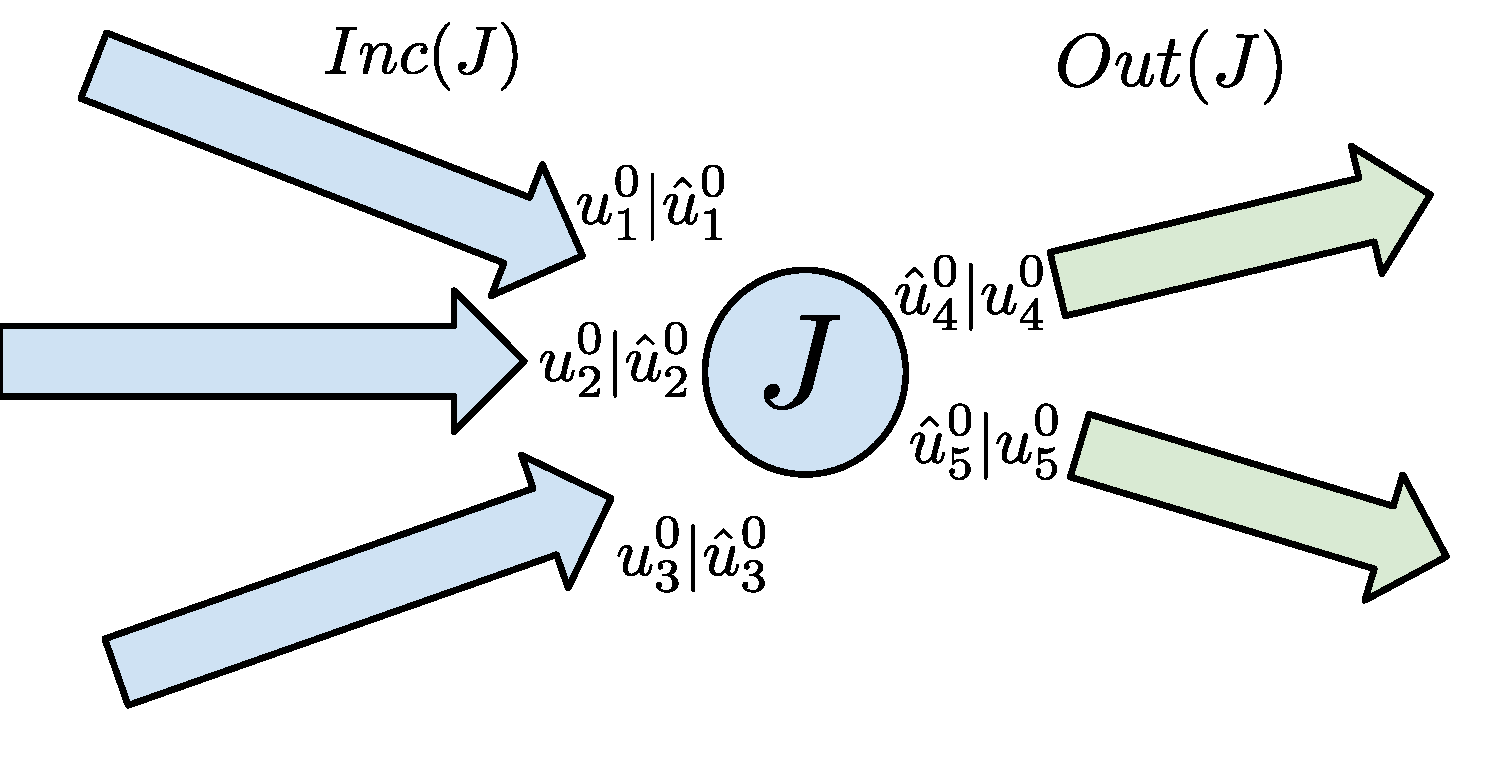
\includegraphics[width=0.5\columnwidth]{presentation/figs-gen/junctions-riemann-rs} 
\par\end{centering}

\caption{Solution of boundary conditions at junction. The boundary conditions
$\tuple{\trace{\cvar}_{1}}{\trace{\cvar}_{5}}$ are produced by applying
the Riemann solver to the initial conditions, $\RS\tuple{\initstate_{1}}{\initstate_{5}}$.\label{fig:Solution-of-boundary}}
\end{figure}


The following conditions are required for a valid Riemann solver as
part of the definition: 
\begin{itemize}
\item The Riemann solver must produce self-similar solutions, i.e. 
\[
\RS\left(\RS\tuple{\initstate_{1}}{\initstate_{\ninc+\nout}}\right)=\RS\tuple{\initstate_{1}}{\initstate_{\ninc+\nout}}=\tuple{\trace{\cvar}_{1}}{\trace{\cvar}_{\ninc+\nout}}
\]

\item All waves produced from the solution to Riemann problems on all links,
generated by the boundary conditions at a junction, must emanate out
from the junction. For example, the solution to the Riemann problem
on an incoming link must produce waves with negative speeds, while
the solution on an outgoing link must produce waves with positive
speed. 
\item The sum of all incoming fluxes must equal the sum of all outgoing
fluxes: 
\[
\sum_{i\in\Inc\left(\jn\right)}f\left(\trace{\cvar}_{\link}\right)=\sum_{j\in\Out\left(\jn\right)}f\left(\trace{\cvar}_{j}\right)
\]



This condition guarantees mass conservation at junctions.

\end{itemize}
The justification for these conditions can be found in~\cite{garavello2006traffic}.


\subsection{Godunov Discretization\label{sub:Godunov-Discretization}}

To approximate a hyperbolic PDE of the form in~(\ref{eq:cons-smooth})
with a discretization in both space and time, we use Godunov's scheme~\cite{godunov1959}.
Given an initial condition that is piecewise-constant, Godunov's scheme
gives a procedure to advance the system one time-step forward. Under
suitable stability conditions, this process can be repeated \emph{ad
infinum }by applying the scheme to the new condition generated from
the previous time-step.

We define a numerical grid using the following notations 
\begin{itemize}
\item $\Delta x$ is the fixed space grid size,
\item $\Delta t$ is the fixed time grid size, chosen with respect to the
The Courant\textendash{}Friedrichs\textendash{}Lewy (CFL) condition%
\footnote{This method can be generalized to non-uniform grid sizes, but is chosen
to be uniform to simplify notation%
}, 
\item $(t^{\tind},\xdis{\xind})=(k\Delta t,\xind\Delta x)$ for $\tind\in\mathbb{N}$
and $\xind\in\mathbb{Z}$ grid points%
\footnote{The CFL condition, $\lambda^{\max}\le\frac{\Delta x}{\Delta t}$,
guarantees that the waves in two neighboring cells do not interact
at the cell boundaries before $\Delta t$. Above $\lambda^{\max}=\underset{a}{\max}|f'\left(a\right)|$
is the maximum absolute wave speed. We assume henceforth that this
condition always holds for the chosen step sizes.%
}. For a link $\link\in\links$ with space domain $\left(0,\length_{\link}\right)$,
$\xind$ takes values in $\intrange 0{\length_{\link}^{\Delta}}$.
\end{itemize}
For a function $\dvar$ defined at the grid we write $\discrete{\xind}{\tind}=\dvar(t^{\tind},\xdis{\xind})$
for $\tind,\xind$ varying on a subset of $\mathbb{N}$ and $\mathbb{Z}$.
The space discretization scheme is depicted for a link $\link\in\links$
in Figure~\ref{fig:Space-discretization-for}
\begin{figure}
\begin{centering}
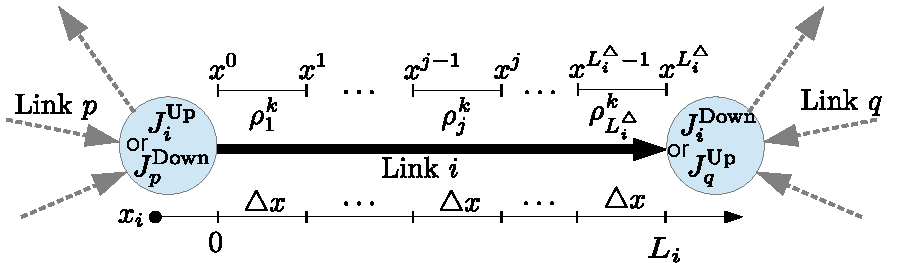
\includegraphics[width=0.6\columnwidth]{figs-gen/dx}
\par\end{centering}

\caption{Space discretization for a link $\link\in\links$. Step size is uniform
$\Delta x$, with discrete value $\discrete{\xind}{\tind}$ representing
the state between $x^{\xind-1}$ and $x^{\xind}$.\label{fig:Space-discretization-for}}


\end{figure}
.


\paragraph{Godunov scheme for a single link.}

Consider a hyperbolic equation together with an initial condition
as expressed in~(\ref{eq:cauchy}). A solution of the discretized
problem is constructed by taking a piecewise constant approximation
of the initial data $\initvar{\dvar}^{\Delta}$ and then constructing
the solution iteratively from the approximate initial data as in~(\ref{eq:godproj}).
\begin{equation}
\discrete{\xind}{\tind}\approxeq\dfrac{1}{\Delta x}\int_{\xdis{\xind-\frac{1}{2}}}^{\xdis{\xind+\frac{1}{2}}}\dvar^{\Delta}(t^{k},x)dx.\label{eq:godproj}
\end{equation}


where $\cvar^{\Delta}\left(t,x\right)$ is an exact solution of~(\ref{eq:cauchy})
with initial condition $\initstate^{\Delta}$.

Since $\cvar^{\Delta}$ in~(\ref{eq:godproj}) is an exact solution
of~(\ref{eq:cons-smooth}) we can use the Gauss-Green formula to
compute this value. Under the CFL condition, the solutions are locally
given by the solutions of the Riemann problems and, in particular,
the flux at $x=\xdis{\xind+\frac{1}{2}}$ for $t\in(t^{k},t^{k+1})$
is given by 
\[
f(\cvar(t,\xdis{\xind}))=f(W_{R}(0;\discrete{\xind}{\tind},\discrete{\xind+1}{\tind})).
\]
This flux solution is depicted in Figure~\ref{fig:Self-similar-solution-for}
\begin{figure}
\begin{centering}
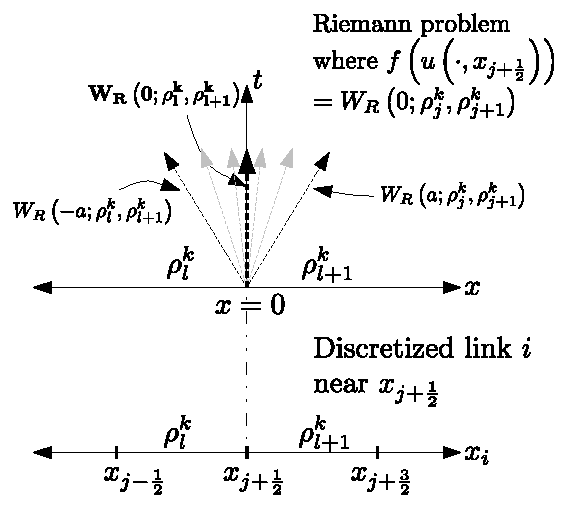
\includegraphics[width=0.5\columnwidth]{figs-gen/dx-to-riemann}
\par\end{centering}

\caption{Self-similar solution for Riemann problem with initial data $\left(\discrete{\xind}{\tind},\discrete{\xind+1}{\tind}\right)$.
The self-similar solution at $\frac{x}{t}=0$ for the top diagram
(i.e. $\ss 0{\discrete{\xind}{\tind}}{\discrete{\xind+1}{\tind}}$),
gives the flux solution to the discretized problem in the bottom diagram.\label{fig:Self-similar-solution-for}}
\end{figure}
.The flux at $x=\xdis{\xind-\frac{1}{2}}$ for $t\in(t^{k},t^{k+1})$
is given by 
\[
f(\cvar(t,\xdis{\xind-\frac{1}{2}}))=f(W_{R}(0;\discrete{\xind-1}{\tind},\discrete{\xind}{\tind})).
\]
As the flux is constant at $x=0$ for the Riemann problem, we can
put it out of the integral and, setting $\god(u,v)=f(W_{R}(0;u,v))$,
the scheme can be written as 
\begin{equation}
\discrete{\xind}{\tind+1}=\discrete{\xind}{\tind}-\frac{\Delta t}{\Delta x}(\god(\discrete{\xind}{\tind},\discrete{\xind+1}{\tind})-\god(\discrete{\xind-1}{\tind},\discrete{\xind}{\tind})),\label{eq:godscheme}
\end{equation}
where $g^{G}$ is the numerical flux:

\begin{eqnarray*}
\god: & \mathbb{R}\times\mathbb{R} & \rightarrow\mathbb{R}\\
 & \left(\discrete{\xind}{},\discrete{\xind+1}{}\right) & \mapsto\god\left(\discrete{\xind}{},\discrete{\xind+1}{}\right)=f(W_{R}(0;\discrete{\xind}{},\discrete{\xind+1}{}))
\end{eqnarray*}



\paragraph{Godunov scheme at junctions.\label{par:Godunov-scheme-at}}

The scheme just discussed applies to the case in which a single cell
is adjacent to another single cell. Yet, at junctions, a cell may
share a boundary with more than one cell. A more general Godunov flux
can be derived for such cases. For incoming links near the junction,
we have: 
\begin{align*}
\discrete{\length_{\link}^{\Delta}}{\tind+1}=\discrete{\length_{\link}^{\Delta}}{\tind}-\dfrac{\Delta t}{\Delta x}(f(\trace{\dvar}_{\length_{\link}^{\Delta}}^{\tind})-\god(\discrete{L_{i}^{\Delta}-1}{\tind},\discrete{L_{i}^{\Delta}}{\tind})), &  & \link\in\left\{ 1,\ldots,\ninc\right\} 
\end{align*}
where $\hat{\dvar}_{i}^{\tind}$ is the solution of the Riemann solver
$\RS\tuple{\discrete 1{\tind}}{\discrete{\ninc+\nout}{\tind}}$ for
link $\link$ at the junction. The same can be done for the outgoing
links: 
\begin{align*}
\discrete 1{\tind+1}=\discrete 1{\tind}-\dfrac{\Delta t}{\Delta x}(\god(\discrete 1{\tind},\discrete 2{\tind})-f(\trace{\dvar}_{1}^{\tind})), &  & \link\in\left\{ \ninc+1,\ldots,\ninc+\nout\right\} 
\end{align*}

\begin{rem}
Using the Godunov scheme, each mesh grid at a given $t^{\tind}$ can
be seen as a node for a 1-to-1 junction with one incoming and one
outgoing link. It is therefore more convenient to consider that every
discretized cell is, rather, a link with both an upstream and downstream
junction. Thus, we consider networks in which the state of each link
$\link\in\links$ at a time-step $k\in\intrange 0{\ntime-1}$ is represented
by the single discrete value $\discrete{\link}{\tind}$.
\end{rem}
The previous remark allows us to develop a generalized update step
for all discrete state variables. We first introduce a definition
in order to reduce the cumbersome nature of the preceding notation.
Let the state variables adjacent to a junction $\jn\in\jns$ at a
time-step $\tind\in\intrange 0{\ntime-1}$ be represented as $\juncstate{\jn}{\tind}\defeq\tuple{\discrete{\link_{\jn}^{1}}{\tind}}{\discrete{\link_{\jn}^{\ninc_{\jn}+\nout_{\jn}}}{\tind}}$.
Similarly, we let the solution of a Riemann solver be represented
as $\junctrace{\jn}{}\defeq\RS\left(\juncstate{\jn}{}\right)$. Then,
for a link $\link\in\links$ with upstream and downstream junctions,
$\jup{\link}$ and $\jdown{\link}$, and time-step $\tind\in\left\{ 0,\ldots,\ntime-1\right\} $,
the update step becomes:

\begin{align}
\discrete{\link}{\tind+1} & =\discrete{\link}{\tind}-\dfrac{\Delta t}{\Delta x}\left(f\left(\left(\RS\left(\juncstate{\jdown{\link}}{\tind}\right)\right)_{\link}\right)-f\left(\left(\RS\left(\juncstate{\jup{\link}}{\tind}\right)\right)_{\link}\right)\right)\nonumber \\
 & =\discrete{\link}{\tind}-\dfrac{\Delta t}{\Delta x}\left(f\left(\left(\junctrace{\jdown{\link}}{}\right)_{\link}\right)-f\left(\left(\junctrace{\jup{\link}}{}\right)_{\link}\right)\right)\label{eq:reg-update}
\end{align}


where $\left(s\right)_{i}$ is the $i$th element of the tuple $s$.
This equation is thus a general way of writing the Godunov scheme
in a way which applies everywhere, including at junctions.


\paragraph{Working directly with flux solutions at junctions.\label{par:Composing-the-Riemann}}

The equations can be simplified if we do not explicitly represent
the solution of the Riemann solver, $\junctrace{\jn}{}$, and, instead,
directly calculate the flux solution from the Riemann data. We denote
this direct computation by $\god_{\jn}$, the Godunov flux solution
at a junction:

\begin{eqnarray}
\god_{\jn}: & \mathbb{R}^{\ninc_{\jn}+\nout_{\jn}} & \rightarrow\mathbb{R}^{\ninc_{\jn}+\nout_{\jn}}\nonumber \\
 & \juncstate{\jn}{} & \mapsto f\left(RS\left(\juncstate{\jn}{}\right)\right)=\left(f\left(\trace{\dvar}_{1}\right),\ldots,f\left(\trace{\dvar}_{\ninc+\nout}\right)\right)\label{eq:god-jn}
\end{eqnarray}
This gives a simplified expressions for the update step:

\begin{equation}
\discrete{\link}{\tind+1}=\discrete{\link}{\tind}-\dfrac{\Delta t}{\Delta x}\left(\left(\god_{\jdown{\link}}\left(\juncstate{\jdown{\link}}{\tind}\right)\right)_{\link}-\left(\god_{\jup{\link}}\left(\juncstate{\jup{\link}}{\tind}\right)\right)_{\link}\right)\label{eq:composed-flux}
\end{equation}



\paragraph{Full discrete solution method.\label{par:Full-solution-method}}

We assume a discrete scalar hyperbolic network of PDEs with links
$\links$ and junctions $\jns$, and a known discrete state at time-step
$\tind$, $\left(\initdiscrete_{\link}^{\tind}:\link\in\links\right)$.
The solution method for advancing the discrete system forward one
time-step is given in Algorithm~(\ref{algo:rs-alg}), or alternatively
Algorithm~(\ref{algo:god-alg}).

\begin{algorithm}[H]
\caption{\texttt{Riemann solver update procedure}}


\lstinputlisting[basicstyle={\ttfamily\footnotesize},breaklines=true,label={algo:rs-alg},mathescape=true]{rs-alg}
\end{algorithm}


Algorithm~\ref{algo:rs-alg} takes as input the state at a time-step
$\tind$ for all links $\left(\discrete{\link}{\tind}:\link\in\links\right)$
and returns the state advanced by one time-step $\left(\discrete{\link}{\tind+1}:\link\in\links\right)$.
The algorithm first iterates over all junctions $\jn$, calculating
all the boundary conditions, $\junctrace{\jn}{\tind}$. Then, the
algorithm iterates over all links $\link\in\links$ to compute the
updated state $\discrete{\link}{\tind+1}$ using the previously computed
boundary conditions, as in~\ref{eq:reg-update}.

\begin{algorithm}[h]
\caption{\texttt{Godunov junction flux update procedure}}


\lstinputlisting[basicstyle={\ttfamily\footnotesize},breaklines=true,label={algo:god-alg},mathescape=true]{god-alg}
\end{algorithm}


Algorithm~\ref{algo:god-alg} is similar to Algorithm~\ref{algo:rs-alg},
except that the boundary conditions $\junctrace{\jn}{\tind}$ are
not explicitly computed, but rather the Godunov flux solution is used
to update the state, as in~\ref{eq:composed-flux}. Algorithm~\ref{algo:god-alg}
is more suitable if a Godunov flux solution is derived for solving
junctions, while Algorithm~\ref{algo:rs-alg} is more suitable if
one uses a Riemann solver at junctions.


\subsection{State, control, and governing equations\label{sec:State,-control,-and}}

The rest of the article focuses on controlling systems of the form
in Algorithm~\ref{algo:god-alg} in which some parts of the state
can be controlled directly (for example, in the form of boundary control).
We wish to solve the system in Algorithm~\ref{algo:god-alg} $T$
time-steps forward, i.e. we wish to determine the discrete state values
$\discrete{\link}{\tind}$ for all links $\link\in\links$ and all
time-steps $\tind\in\intrange 0{\ntime-1}$. Furthermore, at each
time-step $\tind$, we assume a set of ``control'' variables $\tuple{\condiscrete 1{\tind}}{\condiscrete{\ncontrols}{\tind}}\in\mathbb{R}^{\ncontrols}$
that influence the solution of the Riemann problems at junctions,
where $\ncontrols$ is the number of controlled values at each time-step,
and each control may be updated at each time-step. We assume that
a control may only influence a subset of junctions, which is a reasonable
assumption if the controls have some spatial locality. Thus, for a
junction $\jn\in\jns$, we assume without loss of generality that
a subset of the control parameters $\tuple{\condiscrete{\cind_{\jn}^{1}}{\tind}}{\condiscrete{\cind_{\jn}^{\ncontrols_{\jn}}}{\tind}}\in\mathbb{R}^{\ncontrols_{\jn}}$
influence the solution of the Riemann solver. Similar to the notation
developed for state variables, for control variables, we define $\junccon{\jn}{\tind}\defeq\tuple{\condiscrete{\cind_{\jn}^{1}}{\tind}}{\condiscrete{\cind_{\jn}^{\ncontrols_{\jn}}}{\tind}}$
as the concatenation of the control variables around the junction
$\jn$. To account for the addition of controls, we modify the Riemann
problem at a junction $\jn\in\jns$ at time-step $\tind$ to be a
function of the current state of connecting links $\juncstate{\jn}{\tind}$,
and the current control parameters $\junccon{\jn}{\tind}$. Then using
the same notation as before, we express the Riemann solver as:

\begin{eqnarray*}
\RS_{\jn}: & \mathbb{R}^{\ninc_{\jn}+\nout_{\jn}}\times\mathbb{R}^{\ncontrols_{\jn}} & \rightarrow\mathbb{R}^{\ninc_{\jn}+\nout_{\jn}}\\
 & \left(\juncstate{\jn}{\tind},\junccon{\jn}{\tind}\right) & \mapsto\RS_{\jn}\left(\juncstate{\jn}{\tind},\junccon{\jn}{\tind}\right)=\junctrace{\jn}{\tind}
\end{eqnarray*}


We represent the entire state of the solved system with the vector
$\state\in\mathbb{R}^{\nlinks\ntime}$, where for $\link\in\links$
and $k\in\intrange 0{\ntime-1}$, we have $\state_{\nlinks k+\link}=\discrete{\link}{\tind}$.
Similarly, we represent the entire control vector by $\control\in\mathbb{R}^{\ncontrols\ntime}$,
where $\control_{\ncontrols\tind+\cind}=\condiscrete{\cind}{\tind}$.

For each state variable $\discrete{\link}{\tind}$, write the corresponding
update equation $\syseq_{\link}^{\tind}$:

\begin{eqnarray*}
\syseq_{\link}^{\tind}: & \mathbb{R}^{\nlinks\ntime}\times\mathbb{R}^{\ncontrols\ntime} & \rightarrow\mathbb{R}\\
 & \left(\state,\control\right) & \mapsto\syseq_{\link}^{\tind}\left(\state,\control\right)=0
\end{eqnarray*}


This takes the following form:

\begin{eqnarray}
h_{\link}^{0}\left(\state,\control\right)=\discrete{\link}0-\initdiscrete_{\link} & =0\label{eq:init-ge}\\
\syseq_{\link}^{\tind}\left(\state,\control\right)=\discrete{\link}{\tind}-\discrete{\link}{\tind-1}+\frac{\Delta t}{L_{\link}}f\left(\RS_{\jdown{\link}}\left(\juncstate{\jdown{\link}}{\tind-1},\junccon{\jdown{\link}}{\tind-1}\right)\right)_{\link}\nonumber \\
-\frac{\Delta t}{L_{\link}}f\left(\RS_{\jup{\link}}\left(\juncstate{\jup{\link}}{\tind-1},\junccon{\jup{\link}}{\tind-1}\right)\right)_{\link} & =0 & \forall k\in\intrange 2{\ntime-1},\label{eq:main-ge}
\end{eqnarray}
or in terms of the Godunov junction flux:

\begin{eqnarray}
\syseq_{\link}^{\tind}\left(\state,\control\right)= & \discrete{\link}{\tind}-\discrete{\link}{\tind-1} & +\dfrac{\Delta t}{\Delta x}\left(\god_{\jdown{\link}}\left(\juncstate{\jdown{\link}}{\tind},\junccon{\jdown{\link}}{\tind-1}\right)\right)_{\link}\nonumber \\
 &  & -\dfrac{\Delta t}{\Delta x}\left(\god_{\jup{\link}}\left(\juncstate{\jup{\link}}{\tind},\junccon{\jup{\link}}{\tind-1}\right)\right)_{\link}\label{eq:syseq-god}
\end{eqnarray}
for all links $\link\in\links$, where $\initdiscrete_{\link}$ is
the initial condition for link $\link$. Thus, we can construct a
system of $\nlinks T$ governing equations $H\left(\state,\control\right)=0$,
where the $h_{\link,k}$ is the equation in $H$ at index $\nlinks k+\link$,
identical to the ordering of the corresponding discrete state variable. 


\section{Adjoint based flow optimization\label{sec:Adjoint-method}}


\subsection{Optimal control problem formulation\label{par:Optimization-Problem}}

In addition to our governing equations $\sys\left(\state,\control\right)=0$,
we also introduce a cost function $\cost$, which we assume to be
in $C^{2}$:

\begin{eqnarray*}
	\cost: & \mathbb{R}^{\nlinks T}\times\mathbb{R}^{\ncontrols T} & \rightarrow\mathbb{R}\\
	& \left(\state,\control\right) & \mapsto\cost\left(\state,\control\right)
\end{eqnarray*}


which returns a scalar that serves as a metric of performance of the
state and control values of the system. We wish to minimize the quantity
$\cost$ over the set of control parameters $\control$, while constraining
the state of the system to satisfy the governing equations $\sys\left(\state,\control\right)=0$,
which is, again, the concatenated version of~\eqref{eq:main-ge} or~\eqref{eq:syseq-god}.
We summarize this with the following optimization problem:

\begin{eqnarray}
	\underset{\control}{\min} & \cost\left(\state,\control\right)\nonumber \\
	\text{subject to:} & \sys\left(\state,\control\right)=0\label{eq:op-problem}
\end{eqnarray}


Both the cost function and governing equations may be non-convex in
this problem.


\subsection{Calculating the gradient\label{par:Calculating-the-gradient}}

We wish to use gradient information in order to find control values
$\control^{*}$ that give locally optimal costs $\cost^{*}=\cost\left(\state\left(\control^{*}\right),\control^{*}\right)$.
Since there may exist many local minima for this optimization problem~\eqref{eq:op-problem}
(which is non-convex in general), gradient\emph{ }methods do not guarantee
global optimality of $\control^{*}$\emph{. }Still, nonlinear optimization
methods such as interior point optimization utilize gradient information
to improve performance~\cite{Andreas2005}.

In a descent algorithm, the optimization procedure will have to descend
a cost function, by coupling the gradient, which, at a nominal point
$\left(\nominal{\state},\nominal{\control}\right)$ is given by:

\begin{equation}
	d_{\control}\cost\left(\nominal{\state},\nominal{\control}\right)=\evaluate{\pfrac{\cost\text{\ensuremath{\left(\state,\control\right)}}}{\state}}{\nominal{\state},\nominal{\control}}\Dfrac{\state}{\control}+\evaluate{\pfrac{\cost\text{\ensuremath{\left(\state,\control\right)}}}{\control}}{\nominal{\state},\nominal{\control}}\label{eq:j-v}
\end{equation}


The main difficulty is to compute the term $\Dfrac{\state}{\control}$.
Next we take advantage of the fact that the derivative of $H\left(\state,\control\right)$
with respect to $\control$ is equal to zero along trajectories of
the system:

\begin{equation}
	d_{\control}\sys\left(\nominal{\state},\nominal{\control}\right)=\evaluate{\pfrac{\sys\text{\ensuremath{\left(\state,\control\right)}}}{\state}}{\nominal{\state},\nominal{\control}}\Dfrac{\state}{\control}+\evaluate{\pfrac{\sys\text{\ensuremath{\left(\state,\control\right)}}}{\control}}{\nominal{\state},\nominal{\control}}=0\label{eq:h-v}
\end{equation}


The partial derivative terms, $\Hx\in\mathbb{R}^{\nlinks\ntime\times\nlinks\ntime}$,
$\Hu\in\mathbb{R}^{\nlinks\ntime\times\ncontrols\ntime}$, $\Jx\in\mathbb{R}^{\nlinks\ntime}$,
and $\Ju\in\mathbb{R}^{\ncontrols\ntime}$, can all be evaluated (more
details provided in Section~\ref{sub:Evaluating--and}) and then
treated as constant matrices. Thus, in order to evaluate $d_{\control}\cost\left(\nominal{\state},\nominal{\control}\right)\in\mathbb{R}^{\ncontrols\ntime}$,
we must solve a coupled system of matrix equations.
\begin{note}
	In~\eqref{eq:h-v}, $\Hx$ and $\Hu$ might not necessarily by defined,
	either because $f$ itself is not smooth (note that we took $f$ to
	be $C^{2}$ to avoid this problem), and/or because $\god$ is not
	smooth. The derivations below are valid when the partials $\Hx$ and
	$\Hu$ can indeed be taken. There are several settings in which the
	conditions for differentiability are satisfied, see in particular~\cite{Gugat2005,Flasskamp2012}.
\end{note}

\paragraph{Forward system.\label{par:Forward-system}}

If we solve for $\Dfrac{\state}{\control}\in\mathbb{R}^{\nlinks\ntime\times\ncontrols\ntime}$
in~\eqref{eq:h-v}, which we call the \emph{forward system}:

\[
	\Hx\Dfrac{\state}{\control}=-\Hu,
\]


then we can substitute the solved value for $\Dfrac{\state}{\control}$
into~\eqref{eq:j-v} to obtain the full expression for the gradient.
Section~\ref{sub:Evaluating--and} below gives details on the invertibility
of $\Hx$, guaranteeing a solution for $\Dfrac{\state}{\control}$.


\paragraph{Adjoint system.\label{par:Adjoint-system}}

Instead of evaluating $\Dfrac{\state}{\control}$ directly, the adjoint
method instead solves the following system, called the adjoint system,
for a new unknown variable $\lambda\in\mathbb{R}^{\nlinks\ntime}$
(called the adjoint variable):

\begin{equation}
	\Hx^{T}\lambda=-\Jx^{T}\label{eq:adjoint}
\end{equation}
Then the expression for the gradient becomes:

\begin{equation}
	d_{\control}\cost\left(\nominal{\state},\nominal{\control}\right)=\lambda^{T}\Hu+\Ju\label{eq:adjoint-grad}
\end{equation}
We define $\degree{\state}$ to be the maximum junction degree on
the network:

\begin{equation}
	\degree{\state}=\max_{\jn\in\jns}\left(\ninc_{\jn}+\nout_{\jn}\right),\label{eq:dx}
\end{equation}
and also define $\degree{\control}$ to be the maximum number of constraints
that a single control variable appears in, which is equivalent to:

\begin{equation}
	\degree{\control}=\max_{\condiscrete{}{}\in\control}\sum_{\jn\in\jns:\condiscrete{}{}\in\junccon{\jn}{\tind}}\left(\ninc_{\jn}+\nout_{\jn}\right)\label{eq:dv}
\end{equation}


Note that $\left\{ \convar\in\junccon{\jn}{\tind}:\jn\in\jns\right\} $
is a $\tind$-dependent set. By convention, junctions are either actuated
or not, so there is no dependency on $\tind$, i.e. if $\exists\tind$
s.t. $\convar\in\junccon{\jn}{\tind}$, then $\forall\tind$, $\convar\in\junccon{\jn}{\tind}$.

Using these definitions, we show later in Section~\ref{sub:Complexity-of-solving}
how the complexity of computing the gradient is reduced from $O(\degree{\state}\nlinks\ncontrols\ntime^{2})$
to $O(\ntime\left(\degree{\state}\nlinks+\degree{\control}\ncontrols\right))$
by considering the adjoint method over the forward method.

A graphical depiction of $D_{\state}$ and $D_{\control}$ are given
in Figure~\ref{fig:Depicting--and}
\begin{figure}
	\begin{centering}
		\subfloat[\label{fig:genneta}]{\begin{centering}
			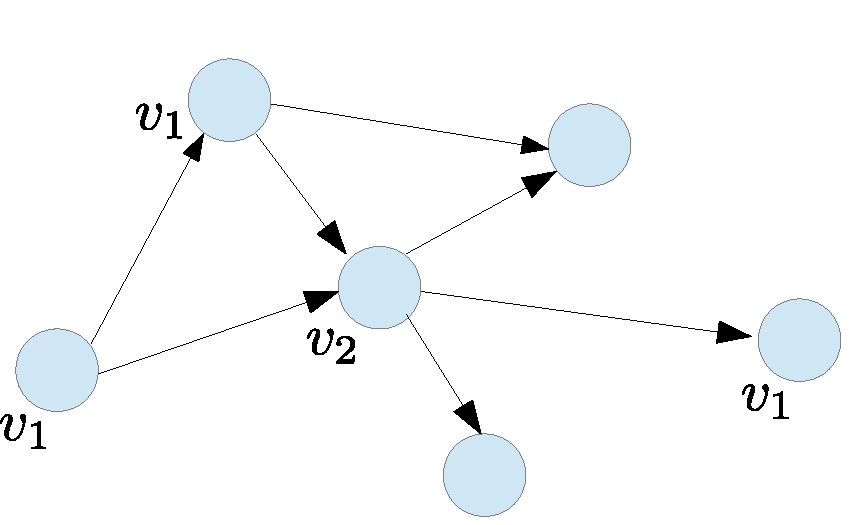
\includegraphics[width=0.33\columnwidth]{figs-gen/gen-net}
			\par\end{centering}
						
			}\subfloat[\label{fig:gennetb}]{\begin{centering}
			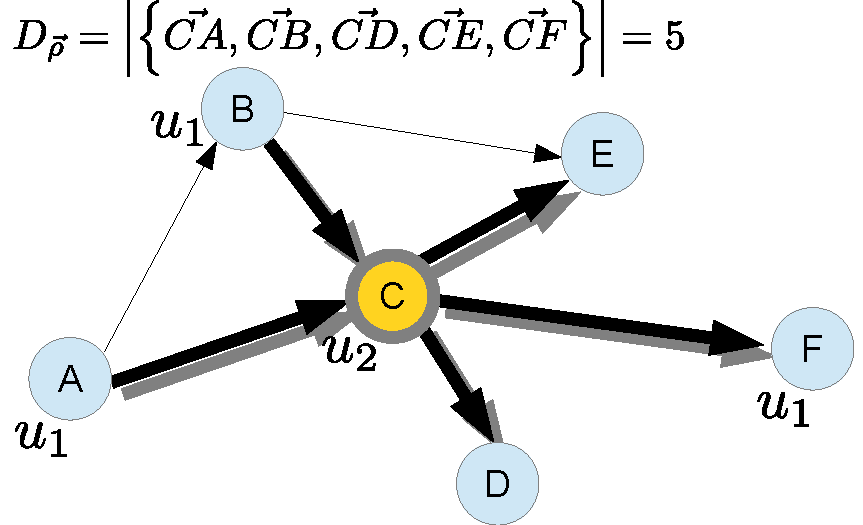
\includegraphics[width=0.33\columnwidth]{figs-gen/gen-net-dx}
			\par\end{centering}
						
			}\subfloat[\label{fig:gennetc}]{\begin{centering}
			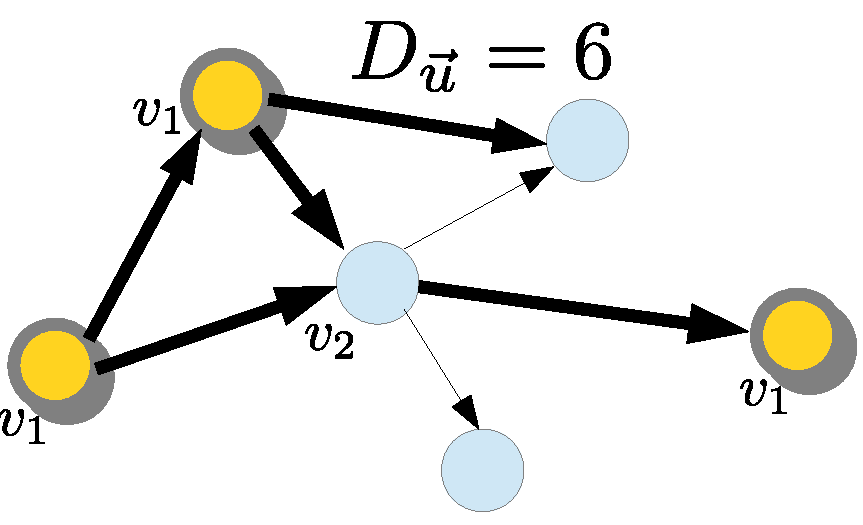
\includegraphics[width=0.33\columnwidth]{figs-gen/gen-net-dv}
			\par\end{centering}
						
		}
		\par\end{centering}
				
		\caption{Depiction of $D_{\state}$ and $D_{v}$ for an arbitrary graph. Figure~\ref{fig:genneta}
			shows the underlying graphical structure for an arbitrary PDE network.
			Some control parameter $\convar_{1}$ has influence over junctions
			$A$, $B$, and $F$, while another control parameter $\convar_{2}$
			has influence over only junction $C$. Figure~\ref{fig:gennetb}
			depicts the center junction having the largest number of connecting
			edges, thus giving $D_{\state}=5$. Figure~\ref{fig:gennetc} shows
			that control parameter $\convar_{1}$ influences three junctions with
			sum of junctions degrees equal to six, which is maximal over the other
			control parameter $\convar_{2}$. leading to the result $D_{\control}=6$.
			Note that in Figure~\ref{fig:gennetc}, the link going from junction
			$A$ to junction $B$ is counted twice: once as an outgoing link $\vec{AB}$
			and once as in incoming link $\vec{BA}$.\label{fig:Depicting--and}}
		\end{figure}
		.Freeway networks are usually considered to have topologies that are
		nearly planar, leading to junctions degrees which typically do not
		exceed 3 or 4, regardless of the total number of links. Also, from
		the locality argument for control variables in Section~(\ref{sec:State,-control,-and}),
		a single control variable's influence over state variables will not
		grow with the size of the network. Since the $\degree{\state}$ and
		$\degree{\control}$ typically do not grow with $\nlinks\ntime$ or
		$\ncontrols\ntime$ for freeway networks, the complexity of evaluating
		the gradient for such networks can be considered linear for the adjoint
		method.
				
				
		\subsection{Evaluating the partial derivatives\label{sub:Evaluating--and}}
				
		While no assumptions are made about the sparsity of the cost function
		$\cost$, the networked-structure of the PDE system and the Godunov
		discretization scheme allows us to say more about the structure and
		sparsity of $\Hx$ and $\Hu$.
				
				
		\paragraph{Partial derivative expressions.}
				
		Given that the governing equations require the evaluation of a Riemann
		solver at each step, we detail some of the necessary computational
		steps in evaluating the $\Hx$ and $\Hu$ matrices. 
				
		If we consider a particular governing equation $\syseq_{\link}^{\tind}\left(\state,\control\right)=0$,
		then we may determine the partial term with respect to $\discrete jl\in\state$
		by applying the chain rule:
				
		\begin{align}
			\pfrac{\syseq_{\link}^{\tind}}{\discrete jl}=\pfrac{\discrete{\link}{\tind}}{\discrete jl}-\pfrac{\discrete{\link}{\tind-1}}{\discrete jl} & +\frac{\Delta t}{L_{i}}f'\left(\RS_{\jdown{\link}}\left(\juncstate{\jdown{\link}}{\tind-1},\junccon{\jdown{\link}}{\tind-1}\right)_{\link}\right)\pfrac{}{\discrete jl}\left(\RS_{\jdown{\link}}\left(\juncstate{\jdown{\link}}{\tind-1},\junccon{\jdown{\link}}{\tind-1}\right)_{\link}\right)\label{eq:dhdufull} \\
			                                                                                                                                           & -\frac{\Delta t}{L_{i}}f'\left(\RS_{\jup{\link}}\left(\juncstate{\jup{\link}}{\tind-1},\junccon{\jup{\link}}{\tind-1}\right)_{\link}\right)\pfrac{}{\discrete jl}\left(\RS_{\jup{\link}}\left(\juncstate{\jup{\link}}{\tind-1},\junccon{\jup{\link}}{\tind-1}\right)_{\link}\right)\nonumber                       
		\end{align}
				
				
		or if we consider the composed Riemann flux solver $\god_{\jn}$ in~\eqref{eq:god-jn}:
				
		\begin{equation}
			\pfrac{\syseq_{\link}^{\tind}}{\discrete jl}=\pfrac{\discrete{\link}{\tind}}{\discrete jl}-\pfrac{\discrete{\link}{\tind-1}}{\discrete jl}+\frac{\Delta t}{L_{i}}\left(\pfrac{}{\discrete jl}\left(\god_{\jdown{\link}}\left(\juncstate{\jdown{\link}}{\tind-1},\junccon{\jdown{\link}}{\tind-1}\right)\right)_{\link}-\pfrac{}{\discrete jl}\left(\god_{\jup{\link}}\left(\juncstate{\jup{\link}}{\tind-1},\junccon{\jup{\link}}{\tind-1}\right)\right)_{\link}\right)\label{eq:dhdugod}
		\end{equation}
				
				
		A diagram of the structure of the $\Hx$ matrix is given in Figure~(\ref{fig:partial-ordering}).
		\begin{figure}
			\subfloat[\label{fig:partial-ordering}Ordering of the partial derivative terms.
				Constraints and state variables are clustered first by time, and then
				by cell index.]{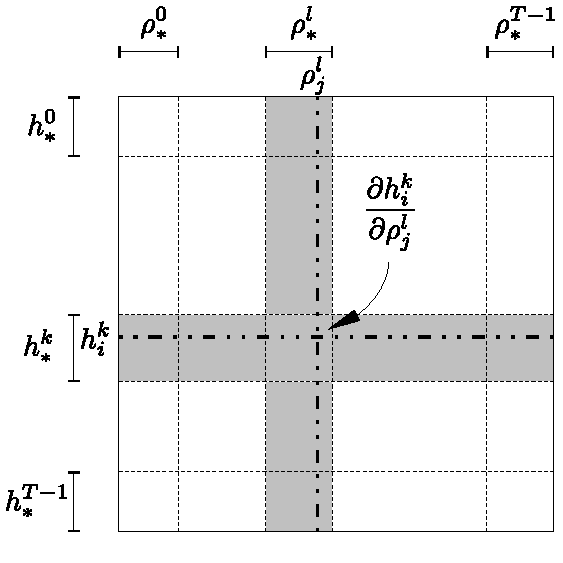
\includegraphics[width=0.45\columnwidth]{figs-gen/dstate}
												
						}\texttt{\hfill{}}\subfloat[\label{fig:sparsity-diagram}Sparsity structure of the $\Hx$ matrix.
				Besides the diagonal blocks, which are identity matrices, blocks where
				$l\neq\tind-1$ are zero.]{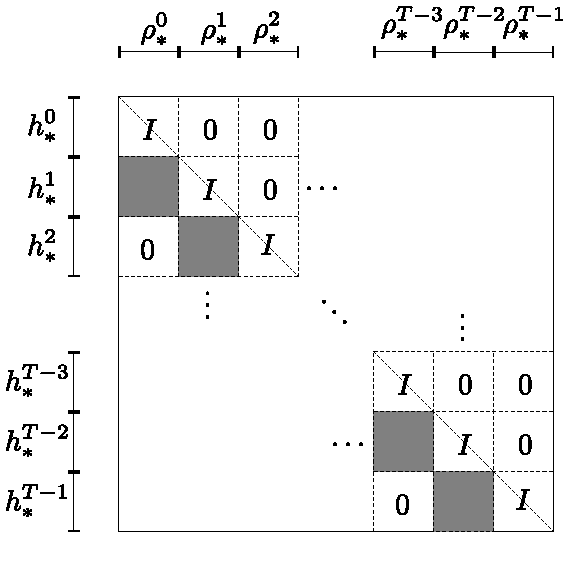
\includegraphics[width=0.45\columnwidth]{figs-gen/sparsity-two}
												
						\texttt{}
												
					}
										
					\caption{Structure of the $\Hx$ matrix.}
										
										
				\end{figure}
				Similarly for $H_{v}$, we take a control parameter $\condiscrete jl\in\control$,
				and derive the expression:
								
				\begin{align}
					\pfrac{\syseq_{\link}^{\tind}}{\condiscrete jl}= & +\frac{\Delta t}{L_{i}}f'\left(\RS_{\jdown{\link}}\left(\juncstate{\jdown{\link}}{\tind-1},\junccon{\jdown{\link}}{\tind-1}\right)_{\link}\right)\pfrac{}{\condiscrete jl}\left(\RS_{\jdown{\link}}\left(\juncstate{\jdown{\link}}{\tind-1},\junccon{\jdown{\link}}{\tind-1}\right)_{\link}\right)\label{eq:dhdvfull} \\
					                                                 & -\frac{\Delta t}{L_{i}}f'\left(\RS_{\jup{\link}}\left(\juncstate{\jup{\link}}{\tind-1},\junccon{\jup{\link}}{\tind-1}\right)_{\link}\right)\pfrac{}{\condiscrete jl}\left(\RS_{\jup{\link}}\left(\juncstate{\jup{\link}}{\tind-1},\junccon{\jup{\link}}{\tind-1}\right)_{\link}\right)\nonumber                       
				\end{align}
								
								
				or for the composed Godunov junction flux solver $\god_{\jn}$:
								
				\begin{equation}
					\pfrac{\syseq_{\link}^{\tind}}{\condiscrete jl}=\frac{\Delta t}{L_{i}}\left(\pfrac{}{\condiscrete jl}\left(\god_{\jdown{\link}}\left(\juncstate{\jdown{\link}}{\tind-1},\junccon{\jdown{\link}}{\tind-1}\right)\right)_{\link}-\pfrac{}{\condiscrete jl}\left(\god_{\jup{\link}}\left(\juncstate{\jup{\link}}{\tind-1},\junccon{\jup{\link}}{\tind-1}\right)\right)_{\link}\right)\label{eqdhdvgod}
				\end{equation}
								
								
				Analyzing~\eqref{eq:dhdufull}, the only partial terms that are not
				trivial to compute are $\pfrac{}{\discrete jl}\left(\RS_{\jdown{\link}}\left(\juncstate{\jdown{\link}}{\tind-1},\junccon{\jdown{\link}}{\tind-1}\right)_{\link}\right)$
				and $\pfrac{}{\discrete jl}\left(\RS_{\jup{\link}}\left(\juncstate{\jup{\link}}{\tind-1},\junccon{\jup{\link}}{\tind-1}\right)_{\link}\right)$.
				Similarly for~\eqref{eq:dhdvfull}, the only nontrivial terms are
				$\pfrac{}{\condiscrete jl}\left(\RS_{\jdown{\link}}\left(\juncstate{\jdown{\link}}{\tind-1},\junccon{\jdown{\link}}{\tind-1}\right)_{\link}\right)$
				and $\pfrac{}{\condiscrete jl}\left(\RS_{\jup{\link}}\left(\juncstate{\jup{\link}}{\tind-1},\junccon{\jup{\link}}{\tind-1}\right)_{\link}\right)$.
				Once one obtains the solutions to these partial terms, then one can
				construct the full $\Hx$ and $\Hu$ matrices and use~\eqref{eq:adjoint}
				and~\eqref{eq:adjoint-grad} to obtain the gradient value.
								
				As these expressions are written for a general scalar conservation
				law, the only steps in computing the gradient that are specific to
				a particular conservation law and Riemann solver are computing the
				derivative of the flux function $f$ and the partial derivative terms
				just discussed. These expressions are explicitly calculated for the
				problem of optimal ramp metering in Section~(\ref{sec:Applications-to-Optimal}).
								
								
				\subsection{Complexity of solving gradient via forward method vs. adjoint method\label{sub:Complexity-of-solving}}
								
								
				\paragraph{Structure and sparsity.\label{par:Structure-and-sparsity}}
								
				We can show the lower-triangular structure and invertibility of $\Hx$
				by examining~\eqref{eq:init-ge} and~\eqref{eq:main-ge}. For $\tind\in\intrange 1{\ntime-1}$,
				we have that $\syseq_{\link}^{\tind}$ is only a function of $\discrete{\link}{\tind}$
				and of the state variables from the previous time-step $\tind-1$.
				Thus, based on our ordering scheme in Section~\ref{sec:State,-control,-and}
				of ordering variables by increasing time-step and ordering constraints
				by corresponding variable, we know for $\Hx$, diagonal terms are
				always $1$ and all upper-triangular terms must be zero (since those
				terms correspond to constraints with a dependence of \emph{future}
				values). These two conditions demonstrate both that $\Hx$ is lower-triangular
				and is also invertible due to the identity matrix block-diagonal terms.
								
				Additionally, if we consider taking partial derivatives with respect
				to the variable $\discrete jl$, then we can deduce from Equation~\eqref{eq:main-ge}
				that all partial terms will be zero except for the diagonal term,
				and those terms involving constraints at time $j+1$ with links connecting
				to the downstream and upstream junctions $\jdown j$ and $\jup j$
				respectively. To summarize, $\Hx$ matrices for systems described
				in Section~\ref{sec:State,-control,-and} will be square, invertible,
				lower-triangular and each column will have a maximum cardinality equal
				to $\degree{\state}$ in~\eqref{eq:dx}. The sparsity structure of
				$\Hx$ is depicted in Figure~(\ref{fig:sparsity-diagram}).
								
				Using the same line of argument for maximum cardinality in $\Hx$,
				we can bound the maximum cardinality of each column of $\Hu$. Taking
				a single control variable $\condiscrete jl$, the variable can only
				appear in constraints at time-step $j+1$ that correspond to a link
				that connects to a junction $\jn$ such that $\condiscrete jl\in\junccon{\jn}{l+1}$.
				These conditions give us the expression for $\degree{\control}$ in~\eqref{eq:dv},
				or the maximum cardinality over all columns in $\Hu$.
								
				If we only consider the lower triangular form of $\Hx$, then the
				complexity of solving for the gradient using the forward system is
				$O(\left(\nlinks\ntime\right)^{2}\ncontrols\ntime)$, where the dominating
				term comes from solving~\eqref{eq:j-v}, which requires the solution
				of $\ncontrols\ntime$ separate $\nlinks\ntime\times\nlinks\ntime$
				lower-triangular systems. The lower-triangular system allows for forward
				substitution, we can be solved in $O(\left(\nlinks\ntime\right)^{2})$
				steps, giving the overall complexity $O(\left(\nlinks\ntime\right)^{2}\ncontrols\ntime)$.
				The complexity of computing the gradient via the adjoint method is
				$O(\left(\nlinks\ntime\right)^{2}+\left(\nlinks\ntime\right)\left(\ncontrols\ntime\right))$,
				which is certainly more efficient than the forward-method, as long
				as $\ncontrols\ntime>1$. The efficiency is gained by considering
				that~\eqref{eq:adjoint} only requires the solution of a single $\nlinks\ntime\times\nlinks\ntime$
				\emph{upper}-triangular system (via backward-substitution), followed
				by the multiplication of $\lambda^{T}H_{v}$, an $\nlinks\ntime\times\nlinks\ntime$
				and an $\nlinks\ntime\times\ncontrols\ntime$ matrix in~\eqref{eq:adjoint-grad},
				with a complexity of $O(\left(\nlinks\ntime\right)^{2}+\left(\nlinks\ntime\right)\left(\ncontrols\ntime\right))$.
								
				For the adjoint method, this complexity can be improved upon by considering
				the sparsity of the $\Hx$ and $\Hu$ matrices, as detailed in Section~\ref{par:Structure-and-sparsity}.
				For the backward-substitution step, each entry in the $\lambda$ vector
				is solved by \emph{at most} $\degree{\state}$ multiplications, and
				thus the complexity of solving~\eqref{eq:adjoint} is reduced to
				$O(\degree{\state}\nlinks\ntime)$. Similarly, for the matrix multiplication
				of $\lambda^{T}H_{v}$, while $\lambda$ is not necessarily sparse,
				we know that each entry in the resulting vector requires at most $\degree{\control}$
				multiplications, giving a complexity of $O(\degree{\control}\ncontrols\ntime)$. 
				\begin{prop}
					\textup{The total complexity for the adjoint method on a scalar hyperbolic
						network of PDEs is }$O(\ntime\left(\degree{\state}\nlinks+\degree{\control}\ncontrols\right))$.\end{prop}
				


\section{Applications to Optimal coordinated ramp metering on freeways\label{sec:Applications-to-Optimal}}


\subsection{Formulation of the network model and explicit Riemann solver\label{sub:Formulation-of-the}}


\paragraph{Model.}

Consider a freeway section with links $\links=\intrange 1{2\nlinks}$
with a linear sequence of mainline links $=\intrange{2,4}{2\nlinks}$
and connecting onramp links $=\intrange{1,3}{2\nlinks-1}$. At discrete
time $t=\tind\Delta t,0\le\tind\le\ntime-1$, mainline link $2\link\in\links,i\in\intrange 1{\nlinks}$
has a downstream junction $\jdown{2\link}=\jup{2\left(\link+1\right)}$
and an upstream junction $\jup{2\link}=\jdown{2\left(\link-1\right)}$,
while onramp $2\link-1\in\links,i\in\intrange 1{\nlinks}$ has a downstream
junction $\jdown{2\link-1}=\jup{2\link}=\jdown{2\left(\link-1\right)}$
and an upstream junction $\jup{2\link-1}$.

The offramp directly downstream of link $2\link,i\in\intrange 1{\nlinks}$
has, at time-step $\tind$, a split ratio $\splitratio_{2\link}^{\tind}$
representing the ratio of cars which stay on the freeway over the
total cars leaving the upstream mainline of junction $\jdown{2\link}$.
The model assumes that all flux from onramp $2\link-1$ enters downstream
mainline $2\link$. Since $\jup 2$ is the source of the network,
it has no upstream mainline or offramp, and similarly $\jdown{2\nlinks}$
has no downstream mainline or onramp ($\splitratio_{2\nlinks}^{\tind}=0$).
Each link $\link\in\links$ has a discretized state value $\densitydiscrete{\link}{\tind}\in\mathbb{R}$
at each time-step $\tind\in\intrange 0{\ntime-1}$, that represents
the density of vehicles on the link. These values are depicted in
Figure~\ref{fig:Freeway-network-junction}. Junctions that have no
onramps can be effectively represented by adding an onramp with no
demand while junctions with no offramps can be represented by setting
the split ratio to 1.
\begin{figure}
\begin{centering}
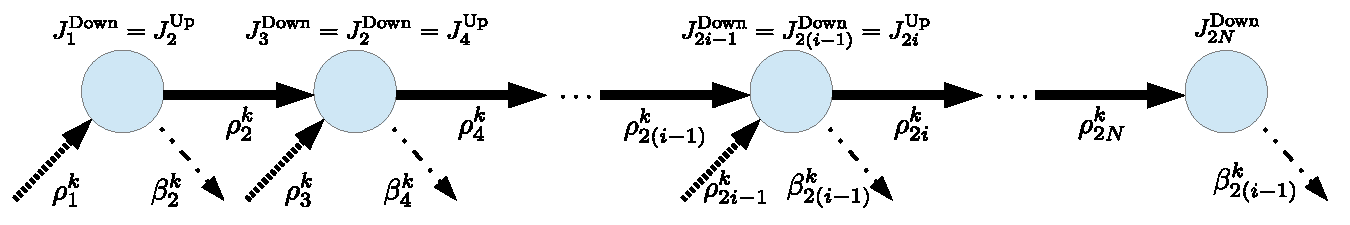
\includegraphics[width=1\columnwidth]{figs-gen/rm-junction-2}
\par\end{centering}

\caption{Freeway network model. For a junction $\jdown{2\link-1}=\jdown{2\left(\link-1\right)}=\jup{2\link}$
at time-step $\tind\in\intrange 0{\ntime-1}$, the upstream mainline
density are represented by $\densitydiscrete{2\left(\link-1\right)}{\tind}$,
the downstream mainline density by $\densitydiscrete{2\link}{\tind}$,
the onramp density by $\densitydiscrete{2\link-1}{\tind}$, and the
offramp split ratio by $\splitratio_{2\left(\link-1\right)}^{\tind}$.\label{fig:Freeway-network-junction}}
\end{figure}


The vehicle flow dynamics on all links $\link$ (mainlines, onramps,
and offramps) are modeled using the conservation law governing the
density evolution~(\ref{eq:cons-smooth}), where $\density$ is the
density state, and $f$ is the flux function (or fundamental diagram)
$f\left(\density\right)$. In the context of traffic, this model is
referred to as the Lighthill-Whitham-Richards (LWR) model~\cite{lighthill1955kinematic,richards1956shock}.
The fundamental diagram $f$ is typically assumed to be concave, and
has a bounded domain $\left[0,\density^{\max}\right]$ and a maximum
flux value $F^{\max}$ attained at a critical density $\density^{c}:f\left(\density^{c}\right)=F^{\max}$.
We assume that the fundamental diagram has a trapezoidal form as depicted
in Figure~\ref{fig:Fundamental-diagram-with}. For the remainder
of the article, we instantiate the conservation law in~(\ref{eq:cons-smooth})
with the LWR equation as it applies to traffic flow modeling.\begin{wrapfigure}{o}{0.5\columnwidth}%
\begin{centering}
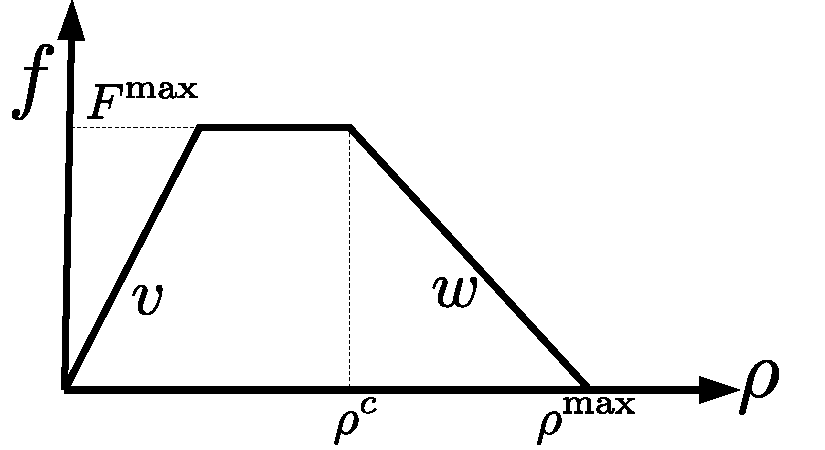
\includegraphics[width=0.4\columnwidth]{figs-gen/fd}
\par\end{centering}

\caption{Fundamental diagram (the name of the flux function in transportation
literature) with free-flow speed $v$, congestion wave speed $w$,
max flux $F^{\max}$, critical density $\density^{c}$, and max density
$\density^{\max}$.\label{fig:Fundamental-diagram-with}}
\end{wrapfigure}%


As control input, an onramp $2\link-1\in\links,\link\in\intrange 1{\nlinks}$
at time-step $k\in\intrange 0{\ntime-1}$ has a metering rate $\ramp_{2\link-1}^{\tind}\in\left[0,1\right]$
which limits the flux of vehicles leaving the onramp. Intuitively,
the metering rate acts as a fractional decrease in the flow leaving
the onramp and entering the mainline freeway. The domain of the metering
control is to force the control to neither impose negative flows nor
send more vehicles than present in a queue. Its mathematical model
is expressed in~(\ref{eq:ramp-eqn}).

For notational simplicity we define the set of densities of links
incident to $\jup{2\link}=\jdown{2\left(\link-1\right)}$ at time-step
$\tind$ as $\juncstate{\jup{2\link}}{\tind}=\left\{ \discrete{2\left(\link-1\right)}{\tind},\discrete{2i-1}{\tind},\discrete{2\link}{\tind}\right\} $.
The offramp is considered to have infinite capacity, and thus has
no bearing on the solution of junction problems. Initial conditions
are handled as in~(\ref{eq:init-ge}), while for $k\in\intrange 1{\ntime-1}$,
the mainline density $\discrete{2\link}{\tind}$ using the Godunov
scheme from~(\ref{eq:main-ge}) is given by:

\begin{eqnarray}
\syseq_{2\link}^{\tind}(\state,\control)= & \discrete{2\link}{\tind}-\discrete{2\link}{\tind-1} & +\dfrac{\Delta t}{\length_{2\link}}\left(\god_{\jdown{2\link}}\left(\juncstate{\jdown{2\link}}{\tind-1},\ramp_{2\link+1}^{\tind-1}\right)\right)_{2\link}\label{eq:rho-update}\\
 &  & -\dfrac{\Delta t}{\length_{2\link}}\left(\god_{\jup{2\link}}\left(\juncstate{\jup{2\link}}{\tind-1},\ramp_{2\link-1}^{\tind-1}\right)\right)_{2\link}\nonumber \\
= & \discrete{2\link}{\tind}-\discrete{2\link}{\tind-1} & +\frac{\Delta t}{\length_{2\link}}\left(\fout{2\link}{\tind-1}-\fin{2\link}{\tind-1}\right)=0
\end{eqnarray}
where we have introduced some substitutions to reduce the notational
burden of this section: $\fout{\link}{\tind}$ is the Godunov flux
at time-step $\tind$ exiting a link $\link$ at the downstream boundary
of the link, and $\fin{\link}{\tind}$ is the Godunov flux entering
the link at the upstream boundary.

We also make the assumption that onramps have infinite capacity and
a free-flow velocity $\ffspeed_{2\link-1}=\frac{\length_{2\link-1}}{\Delta t}$
to prevent the ramp congestion from blocking demand from ever entering
the network. Since the onramp is has no physical length, the length
is chosen arbitrarily and the ``virtual'' velocity chosen above
is chosen to replicate the dynamics in~\cite{Monache2013}. We can
then simplify the onramp update equation to be:

\begin{eqnarray}
\syseq_{2\link-1}^{\tind}(\state,\control) & = & \discrete{2\link-1}{\tind}-\discrete{2\link-1}{\tind-1}+\frac{\Delta t}{\length_{2\link-1}}\left(\left(\god_{\jup{2\link}}\left(\juncstate{\jup{2\link}}{\tind-1},\ramp_{2\link-1}^{\tind-1}\right)\right)_{2\link-1}-\boundaryDemand{2\link-1}{\tind-1}\right)\label{eq:onramp-update}\\
 & = & \discrete{2\link-1}{\tind}-\discrete{2\link-1}{\tind-1}+\frac{\Delta t}{\length_{2\link-1}}\left(\fout{2\link-1}{\tind-1}-\boundaryDemand{2\link-1}{\tind-1}\right)=0
\end{eqnarray}
where $\boundaryDemand{2\link-1}{\tind-1}$ is the onramp \emph{flux
}demand, and the same notational simplification has been used for
the downstream flux. This formulation results in ``strong'' boundary
conditions at the onramps which guarantees all demand enters the network.
Details on weak versus strong boundary conditions can be found in
\cite{Monache2013,Walid,strub2006weak,work2010traffic}.

The onramp model in~(\ref{eq:onramp-update}) differs from~\cite{Monache2013,Walid}
in that we model the onramp as a discretized PDE with an infinite
critical density, while~\cite{Monache2013,Walid} models the onramp
as an ODE ``buffer''. While both models implement strong boundary
conditions, the discretized PDE model makes the freeway network more
aligned with the PDE network framework presented in this article.


\paragraph{Riemann solver.}

For the ramp metering problem, there are many potential Riemann solvers
that satisfy the properties required in Section~\ref{sub:Network-of-PDE's}.
Following the model of \cite{Walid,ML}, for each junction $\jup{2\link}$,
we add two modeling decisions:
\begin{enumerate}
\item The flux solution maximizes the outgoing mainline flux $\fin{2\link}{\tind}$.
\item Subject to (1), the flux solution attempts to satisfy $\fout{2\left(\link-1\right)}{\tind}=p_{2(\link-1)}\fout{2\link-1}{\tind}$,
where $p_{2(\link-1)}\in\mathbb{R}_{+}$ is a merging parameter for
junction $\jdown{2\left(\link-1\right)}$. Since (1) allows multiple
flux solutions at the junction, (2) is necessary to obtain a unique
solution.
\end{enumerate}
This leads to the following system of equations that gives the flux
solution of the Riemann solver at time-step $k\in\intrange 1{\ntime-1}$
and junction $\jup{2\link}$ for $\link\in\intrange 1{\nlinks}$:

\begin{eqnarray}
\demand_{2\left(\link-1\right)}^{\tind} & = & \min\left(\ffspeed_{2\left(i-1\right)}\densitydiscrete{2\left(\link-1\right)}{\tind},F_{2\left(\link-1\right)}^{\max}\right)\label{eq:first-ramp}\\
\supply_{2\link}^{\tind} & = & \min\left(\congspeed_{2i}\left(\density_{2i}^{\max}-\densitydiscrete{2\link}{\tind}\right),F_{2i}^{\max}\right)\label{eq:supply}\\
\rampDemand_{2\link-1}^{\tind} & = & \ramp_{2\link-1}^{\tind}\min\left(\frac{\length_{2\link-1}}{\Delta t}\densitydiscrete{2\link-1}{\tind},F_{2i-1}^{\max}\right)\label{eq:ramp-eqn}\\
\fin{2\link}{\tind} & = & \min\left(\splitratio_{2\left(\link-1\right)}^{\tind}\demand_{2\left(\link-1\right)}^{\tind}+\rampDemand_{2\link-1}^{\tind},\supply_{2\link}^{\tind}\right)\label{eq:fin}\\
\fout{2\left(\link-1\right)}{\tind} & = & \begin{cases}
\demand_{2\left(\link-1\right)}^{\tind} & \frac{p_{2(\link-1)}\fin{2\link}{\tind}}{\splitratio_{2\left(\link-1\right)}^{\tind}\left(1+p_{2(\link-1)}\right)}\ge\demand_{2\left(\link-1\right)}^{\tind}\hfill\text{[Case 1]}\\
\frac{\fin{2\link}{\tind}-\rampDemand_{2\link-1}^{\tind}}{\splitratio_{2\left(\link-1\right)}^{\tind}} & \frac{\fin{2\link}{\tind}}{1+p_{2(\link-1)}}\ge\rampDemand_{2\link-1}^{\tind}\hfill\text{[Case 2}]\\
\frac{p_{2(\link-1)}\fin{2\link}{\tind}}{\left(1+p_{2(\link-1)}\right)\splitratio_{2\left(\link-1\right)}^{\tind}} & \text{otherwise}\hfill[\text{Case 3]}
\end{cases}\label{eq:merge}\\
\fout{2\link-1}{\tind} & = & \fin{2\link}{\tind}-\splitratio_{2\left(\link-1\right)}^{\tind}\fout{2\left(\link-1\right)}{\tind}\label{eq:last-ramp}
\end{eqnarray}
where, for notational simplicity, at the edges of of the range for
$\link$, any undefined state values (e.g. $\densitydiscrete 0{\tind}$)
are assumed to be zero by convention. Equations~(\ref{eq:first-ramp})
and~(\ref{eq:ramp-eqn}) determine the maximum flux that can exit
link $2(\link-1)$ and link $2\link-1$ respectively. Equation~(\ref{eq:supply})
gives the maximum flux allowed into link $2\link$. The actual flux
into link $2\link$, shown in~(\ref{eq:fin}), is given as the minimum
of the ``demand'' from upstream links and ``supply'' of the downstream
link. See~\cite{Monache2013} for more details on the model for this
equation. The flux out of link $2(\link-1)$ is split into three cases
in~(\ref{eq:merge}). The solutions are depicted in Figure~\ref{fig:Godunov-junction-flux},
which demonstrates how the flux solution depends upon the respective
demands and the merging parameter $p_{2\left(\link-1\right)}$. Finally,
Equation~(\ref{eq:last-ramp}) gives the flux out of the onramp $2\link-1$,
which is the difference between the flux into link $2\link$ and the
flux out of link $2\left(\link-1\right)$ the remains on the mainline.
\begin{figure}
\subfloat[Case 1: Priority violated due to limited upstream mainline demand
entering downstream mainline.]{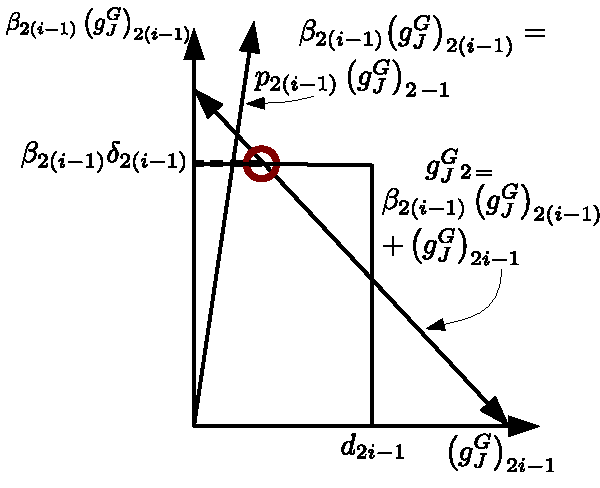
\includegraphics[width=0.3\columnwidth]{figs-gen/flux-sln-1}

}\hfill{}\subfloat[Case 2: Priority violated due to limited onramp demand entering downstream
mainline.]{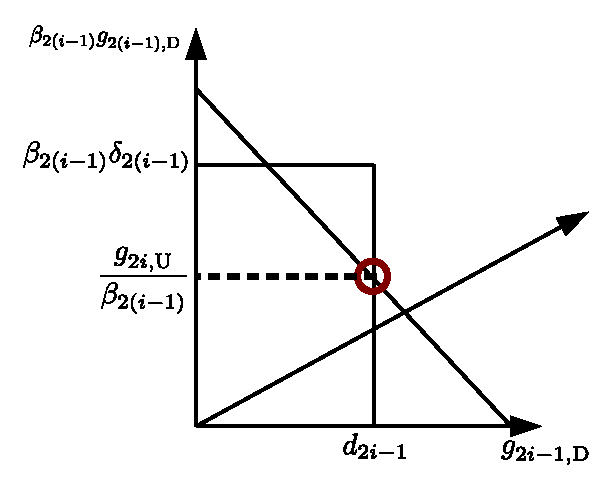
\includegraphics[width=0.3\columnwidth]{figs-gen/flux-sln-2-slim}

}\hfill{}\subfloat[Case 3: Priority rule satisfied due to sufficient demand from both
mainline and onramp.]{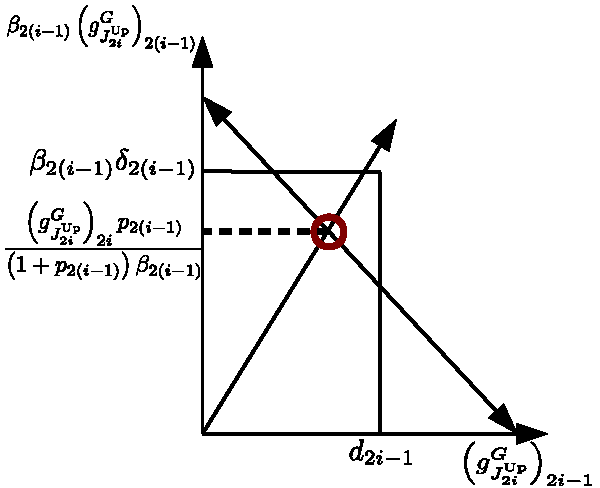
\includegraphics[width=0.3\columnwidth]{figs-gen/flux-sln-3-slim}

}

\caption{Godunov junction flux solution for ramp metering model at junction
$\jup{2\link}$. The rectangular region represents the feasible flux
values for $\splitratio_{2\left(\link-1\right)}\fout{2\left(\link-1\right)}{}$
and $\fout{2\link-1}{}$ as determined by the upstream demand, while
the line with slope\label{fig:Godunov-junction-flux} $\frac{1}{\splitratio_{2\left(\link-1\right)}}$
represents feasible flux values as determined by mass balance. The
$\splitratio_{2\left(\link-1\right)}\fout{2\left(\link-1\right)}{}$
term accounts for only the flux out of link $2\left(\link-1\right)$
that stays on the mainline. The flux solution, represented by the
red circle, is the point on the feasible region that minimizes the
distance from the priority line $\splitratio_{2\left(\link-1\right)}\fout{2\left(\link-1\right)}{}=p_{2(\link-1)}\fout{2\link-1}{}$.}
\end{figure}


For $\tind=0$, the update equation is given by a pre-specified initial
condition, as in~(\ref{eq:init-ge}). Note that the equations can
be solved sequentially via forward substitution. Also, we do not include
the flux result for offramps explicitly here since its value has no
bearing on further calculations, and we will henceforth ignore its
calculation. To demonstrate that indeed the flux solution satisfies
the flux conservation property, the offramp flux is trivially determined
to be $\splitratio_{2\left(\link-1\right)}^{\tind}\fout{2\left(\link-1\right)}{\tind}$.


\subsection{Formulation of the optimal control problem}


\paragraph{Optimal coordinated ramp-metering.}

Including the initial conditions as specified in~(\ref{eq:init-ge})
with~(\ref{eq:rho-update}) and~(\ref{eq:onramp-update}) gives
a complete description of the system $\sys\left(\state,\control\right)=0$,
$\state\in\mathbb{R}^{2\nlinks}$, $\control\in\mathbb{R}$, where:

\begin{eqnarray*}
\state_{2\nlinks\tind+\link}\defeq & \densitydiscrete{\link}{\tind} & 1\le i\le2\nlinks,0\le k\le T-1\\
\control_{\nlinks\tind+\link}\defeq & \ramp_{2\link}^{\tind} & 1\le i\le\nlinks,0\le k\le T-1
\end{eqnarray*}


The objective of the control is to minimize the \emph{total travel
time }on the network, expressed by the cost function $\cost$:

\[
\cost\left(\state,\control\right)=\Delta t\sum_{k=1}^{T}\sum_{i=1}^{2\nlinks}L_{i}\densitydiscrete{\link}{\tind}
\]


The optimal coordinated ramp-metering problem can be formulated as
an optimization problem with PDE-network constraints:

\begin{eqnarray}
\min_{\control} & \cost\left(\state,\control\right)\label{eq:full}\\
\text{subject to:} & \sys\left(\state,\control\right) & =0\nonumber \\
 & 0\le\convar\le1 & \forall\convar\in\control\nonumber 
\end{eqnarray}
Since the adjoint method in Section~\ref{sec:Adjoint-method} only
deals with equality constraints, we add barrier penalties to the cost
function~\cite{Boyd2010,Bayen2006}:

\begin{equation}
\tilde{\cost}\left(\state,\control,\epsilon\right)=\cost\left(\state,\control\right)-\barrierTerm\sum_{\convar\in\control}\log\left(\left(1-\convar\right)\left(\convar-0\right)\right)\label{eq:full-tilde}
\end{equation}


As $\barrierTerm\in\mathbb{R}^{+}$ tends to zero, the solution to~(\ref{eq:full-tilde})
will approach the solution to the original problem~(\ref{eq:full}).
Thus we can solve~(\ref{eq:full}) by iteratively solving the augmented
problem:

\begin{eqnarray}
\min_{\control} & \tilde{\cost}\left(\state,\control,\epsilon\right)\label{eq:full-1}\\
\text{subject to:} & \sys\left(\state,\control\right) & =0\nonumber 
\end{eqnarray}


with decreasing values of $\barrierTerm$. As a result, $\tilde{\cost}$
will approach $\cost$ as the number of iterations increases.


\paragraph{Applying the adjoint method.}

To use the adjoint method as described in Section~\ref{sec:Adjoint-method},
we need to compute the partial derivative matrices $\Hx$, $\Hu$,
$\tilde{C}_{\state}$ and $\tilde{C}_{\control}$. Computing the partial
derivatives with respect to the cost function is straight forward:

\begin{eqnarray*}
\pfrac{\tilde{\cost}}{\discrete{\link}{\tind}}= & \Delta tL_{i} & 1\le i\le2\nlinks,0\le k\le T-1\\
\pfrac{\tilde{\cost}}{\ramp_{2\link}^{\tind}}= & \barrierTerm\left(\frac{-1}{1-\ramp_{2\link}^{\tind}}+\frac{1}{\ramp_{2\link}^{\tind}}\right) & 1\le i\le\nlinks,0\le k\le T-1
\end{eqnarray*}


To compute the partial derivatives of $\sys$, we follow the procedure
in Section~\ref{par:Calculating-the-gradient}. For an upstream junction
$\jup{2\link}\in\jns$ and time-step $k\in\intrange 1{\ntime-1}$,
we only need to compute the partial derivatives of the flux solver
$\god_{\jup{2\link}}\left(\juncstate{\jup{2\link}}{\tind},\ramp_{2\link-1}^{\tind}\right)_{\text{}}$
with respect to the adjacent state variables $\juncstate{\jn_{\link}}{\tind}$
and ramp metering control $\ramp_{\link}^{\tind}$. We calculate the
partial derivatives of the functions in~(\ref{eq:first-ramp})-(\ref{eq:last-ramp})
with respect to either a state or control variable$s\in\state\cup\control$:

\begin{eqnarray*}
\pfrac{\demand_{2\left(\link-1\right)}^{\tind}}s & = & \begin{cases}
\ffspeed_{2\left(i-1\right)} & s=\densitydiscrete{2\left(\link-1\right)}{\tind},\ffspeed_{i}\densitydiscrete{2\left(\link-1\right)}{\tind}\le F_{2\left(i-1\right)}^{\max}\\
0 & \text{otherwise}
\end{cases}\\
\pfrac{\supply_{2\link}^{\tind}}s & = & \begin{cases}
-\congspeed_{2i} & s=\densitydiscrete{2\link}{\tind},\congspeed_{2i}\left(\density_{2i}^{\max}-\densitydiscrete{2\link}{\tind}\right)\le F_{2i}^{\max}\\
0 & \text{otherwise}
\end{cases}\\
\pfrac ds & = & \begin{cases}
\ramp_{2\link-1}^{\tind} & s=\densitydiscrete{2\link-1}{\tind},\densitydiscrete{2\link-1}{\tind}\le F_{2\link-1}^{\max}\\
\min\left(\densitydiscrete{2\link-1}{\tind},F_{2i-1}^{\max}\right) & s=\ramp_{2\link-1}^{\tind}\\
0 & \text{otherwise}
\end{cases}\\
\pfrac{}s\fin{2\link}{\tind} & = & \begin{cases}
\splitratio_{2\left(\link-1\right)}^{\tind}\pfrac{\demand_{2\left(\link-1\right)}^{\tind}}s+\pfrac{\rampDemand_{2\left(\link-1\right)}^{\tind}}s & \splitratio_{2\left(\link-1\right)}^{\tind}\demand_{2\left(\link-1\right)}^{\tind}+\rampDemand_{2\link-1}^{\tind}\le\supply_{2\link}^{\tind}\\
\pfrac{\supply_{2\link}^{\tind}}s & \text{otherwise}
\end{cases}\\
\pfrac{}s\fout{2\left(\link-1\right)}{} & = & \begin{cases}
\pfrac{\demand_{2\left(\link-1\right)}^{\tind}}s & \frac{\fin{2\link}{\tind}p_{2(\link-1)}}{1+p_{2(\link-1)}}\ge\frac{\demand_{2\left(\link-1\right)}^{\tind}}{\splitratio_{2\left(\link-1\right)}^{\tind}}\\
\frac{1}{\splitratio_{2\left(\link-1\right)}^{\tind}}\left(\pfrac{}s\fin{2\link}{\tind}-\pfrac{\rampDemand_{2\link-1}^{\tind}}s\right) & \frac{\fin{2\link}{\tind}}{1+p_{2(\link-1)}}\ge\rampDemand_{2\left(\link-1\right)}^{\tind}\\
\frac{p_{2(\link-1)}}{\splitratio_{2\left(\link-1\right)}^{\tind}\left(1+p_{2(\link-1)}\right)}\pfrac{}s\fin{2\link}{\tind} & \text{otherwise}
\end{cases}\\
\pfrac{}s\fout{2\link-1}{} & = & \pfrac{}s\fin{2\link}{\tind}-\splitratio_{2\left(\link-1\right)}^{\tind}\pfrac{}s\fout{2\left(\link-1\right)}{}
\end{eqnarray*}


These expressions fully quantify the partial derivative values needed
in~(\ref{eq:dhdugod}) and~(\ref{eqdhdvgod}). Thus we can construct
the $\Hx$ and $\Hu$ matrices. With these matrices and $\Jx$ and
$\Ju$, we can solve for the adjoint variable $\lambda\in\mathbb{R}^{2\nlinks\ntime}$
in~(\ref{eq:adjoint}) and substitute its value into~\ref{eq:adjoint-grad}
to obtain the gradient of the cost function $\cost$ with respect
to the control parameter $\control$.


\section{Numerical results for model predictive control simulations\label{sec:Numerical-results-for}}

To demonstrate the effectiveness of using the adjoint ramp metering
method to compute gradients, we implemented the algorithm in MATLAB.
The algorithm can then be used as a gradient computation subroutine
inside any descent-method optimization solver that takes advantage
of first-order gradient information. Our implementation makes use
of the open-source \emph{IpOpt} solver~\cite{Andreas2005}. To serve
as comparisons, three other methods were implemented:
\begin{enumerate}
\item No control: the metering rate is set to 1 on all onramps at all times.
\item Alinea~\cite{Papageorgiou1991}: a popular, feedback-based ramp metering
algorithm. Alinea is computationally efficient and decentralized,
making it a popular choice for large networks, but does not take estimated
boundary flow data as input. Since Alinea has a number of tuning parameters,
we perform a \emph{modified} grid-search technique over the different
parameters that scales linearly with the number of onramps, and select
the best-performing parameters. A \emph{full} grid-search approach
scales exponentially with the number of onramps, rendering it infeasible
for moderate-size freeway networks.
\item Descent method without gradient information: in the absence of gradient
information, the descent-method solver will estimate the gradient
by perturbing control parameters and recomputing the objective function.
\end{enumerate}
The descent method proved to be infeasible for even small, synthetic
networks. Running ramp metering on even a network of 4 links over
6 time-steps for only 5 gradient steps took well over 4 minutes. Already,
the method cannot be used in real-time for freeway networks. The comparison
of running times with and without gradient computations is given in
Figure~\ref{fig:Running-time-of}. We do not consider the method
without gradient computations in further results, due to the impractically
large running times, which only becomes worse as the problem scales
to larger networks and time horizons.
\begin{figure}
\begin{centering}
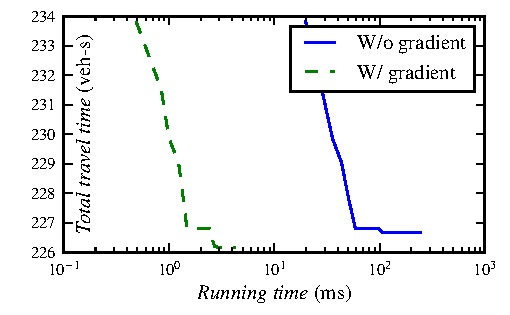
\includegraphics[width=0.65\columnwidth]{images/itergrad}
\par\end{centering}

\caption{Running time of metering algorithm with and without gradient computations.
Network consists of 4 links and 6 time-steps with synthetic boundary
flux data. The method using gradient computations via the adjoint
method converged well before the first step was completed with the
method that used perturbations to compute the gradient.\label{fig:Running-time-of}}
\end{figure}



\subsection{Network\label{sub:Network}}

As input into the optimization problem, we constructed a model of
a 19.4 miles
 stretch of the I15 South freeway in San Diego,
California between San Marcos and Mira Mesa.The network has $\nlinks=$
125
 links, $\ncontrols=$9
 onramps,
with boundary data specified for $\ntime=$ 1800 time-steps,
for a time horizon of 120.0 minutes
 given $\Delta t=$ 4 seconds
.
The network is shown in Figure~\ref{fig:Model-of-section}.
\begin{figure}
\begin{centering}
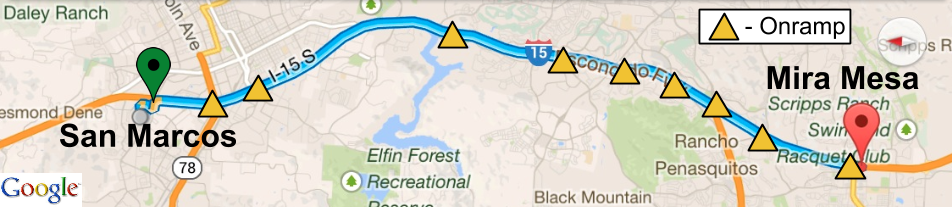
\includegraphics[width=0.7\columnwidth]{images/map}
\par\end{centering}

\caption{Model of section of I15 South in San Diego, California. The freeway
section spanning~19.4 miles was split into~125 links with 9 onramps.\label{fig:Model-of-section}}
\end{figure}


Link length data was obtained using the Scenario Editor software developed
as part of the Connected Corridors project, a collaboration between
UC Berkeley and PATH research institute in Berkeley, California.
Fundamental diagram parameters, split ratios, and boundary data were
also obtained using calibration techniques developed by Connected
Corridors. Densities resulting in free-flow speeds were chosen as
initial conditions on the mainline and onramps. The data used in calibration
was taken from PeMS sensor data during a morning rush hour period,
scaled to generate congested conditions. The input data was chosen
to demonstrate the effectiveness of the adjoint ramp metering method
in a real-world setting. A profile of the mainline and onramps during
a forward simulation of the network is shown in Figure~\ref{fig:Density-and-queue}
under the described boundary conditions.
\begin{figure}
\subfloat[Density profile. The units are the ratio of a link's vehicle density
to a link's critical density. Values less than 1 represent free flow,
while values greater than 1 represent congestion.\label{fig:Density-profile.}]{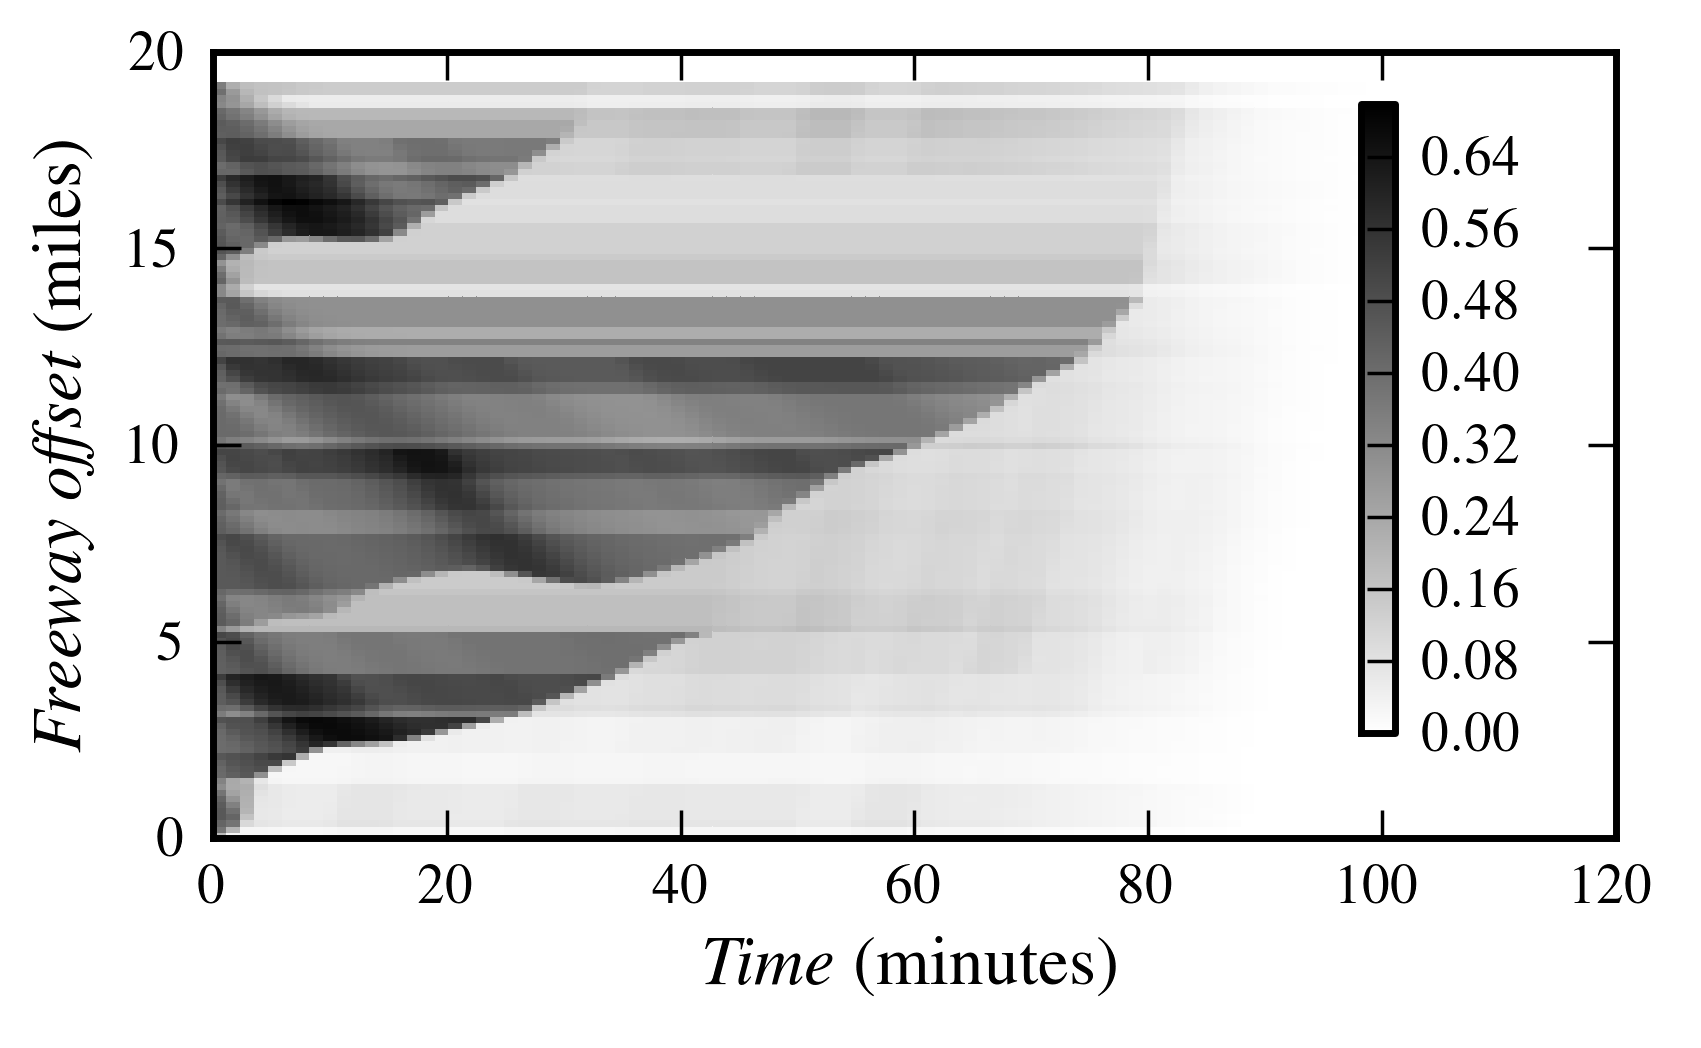
\includegraphics[width=0.45\columnwidth]{images/ncdensity}

}\hfill{}\subfloat[Onramp queue profile in units of vehicles. The onramps are only present
at certain junctions, thus why the nonzero queue lengths are sparse
in this diagram.\label{fig:Density-profile.-2}]{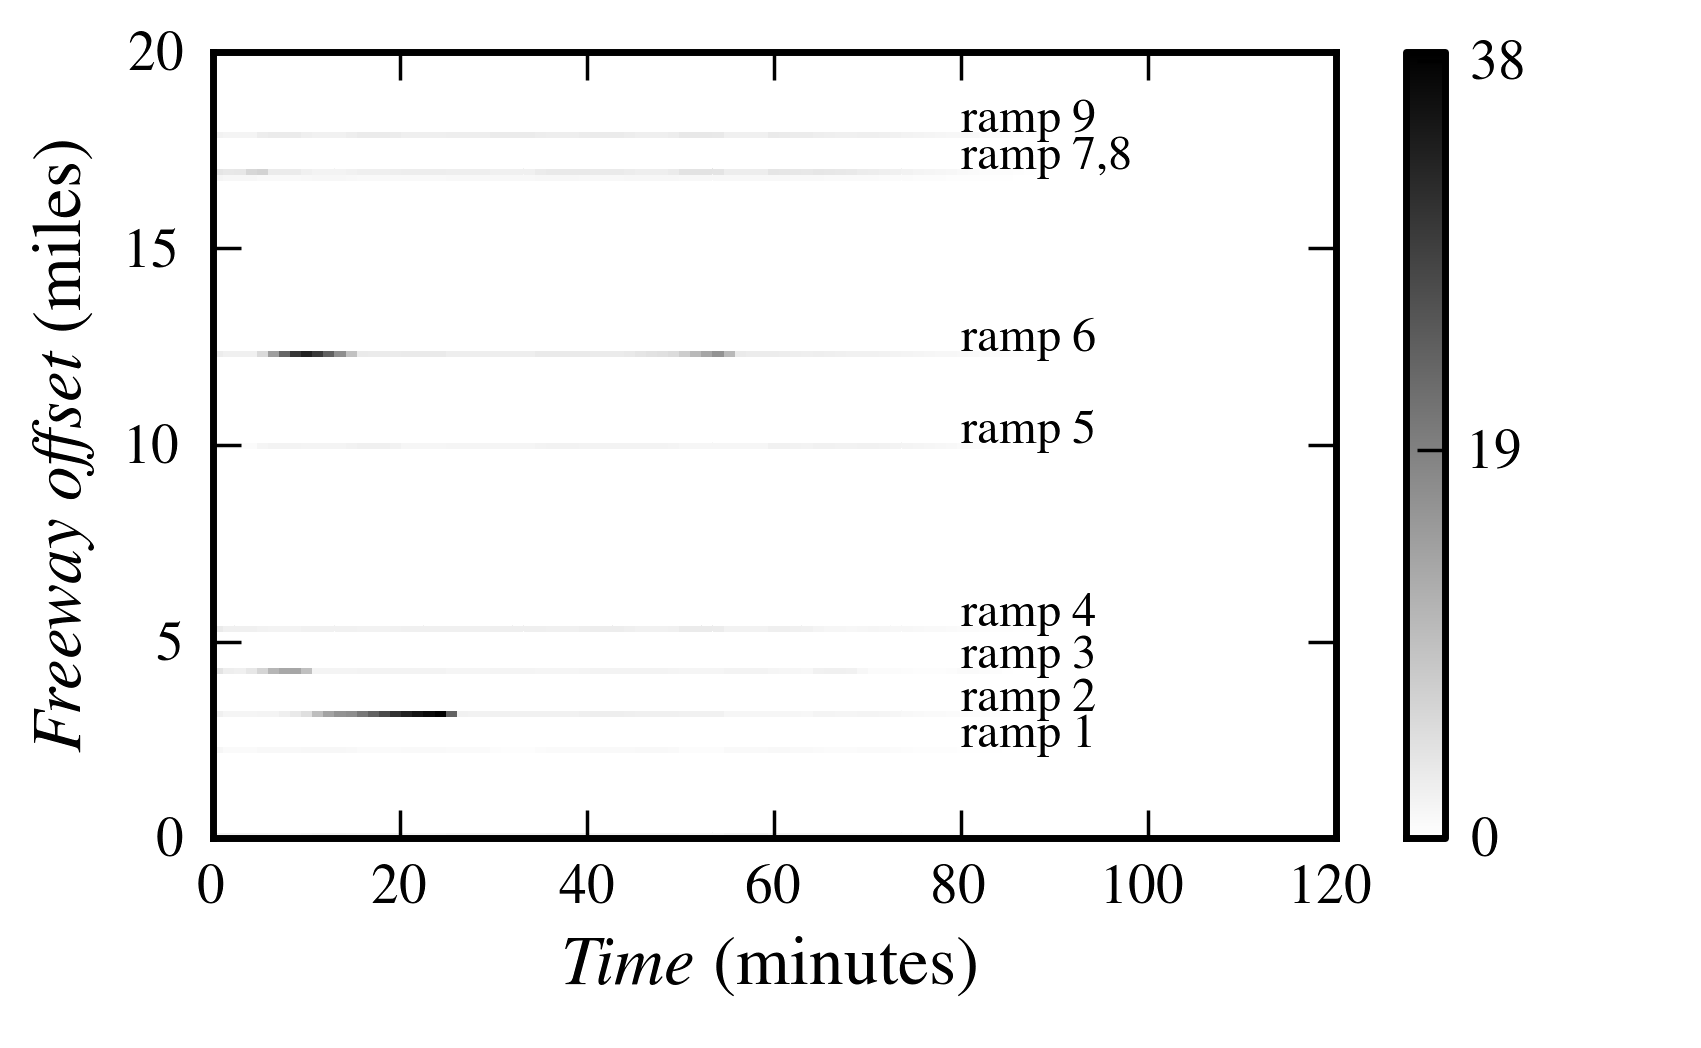
\includegraphics[width=0.45\columnwidth]{images/ncqueue}

}

\caption{Density and queue profile of no-control freeway simulation. In the
first 80 minutes, congestion pockets form on the freeway and queues
form on the onramps, then eventually clear out before 120 minutes.\label{fig:Density-and-queue}}
\end{figure}



\subsection{Finite-horizon optimal control\label{sub:Finite-horizon-optimal-control}}


\paragraph{Experimental setup}

The adjoint ramp metering algorithm is compared to the reactive Alinea
scheme, where we assume perfect boundary conditions and initial conditions
are available. The actual cost used to compare the performances of
the different methods is \emph{delay}, or the total travel time minus
the free-flow total travel time. The free-flow total travel time is
computed by assuming the critical density is infinite for all links,
thus no backwards moving congestion results from high density. The
delay gives an indication of how much improvement is possible, given
that total travel time cannot be zero at optimum.


\paragraph{Results}

\begin{figure}
\subfloat[Density difference profile in units of vehicles per mile.\label{fig:long-sim-density}]{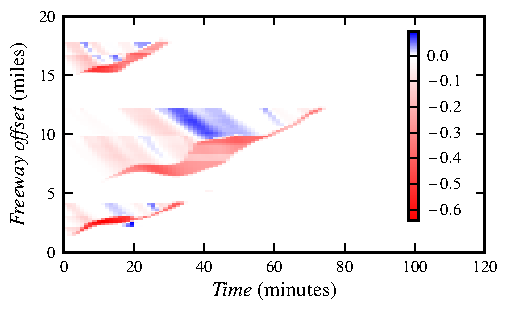
\includegraphics[width=0.45\columnwidth]{images/densdiff}

}\hfill{}\subfloat[Queue difference profile in units of vehicles.\label{fig:long-sim-queue}]{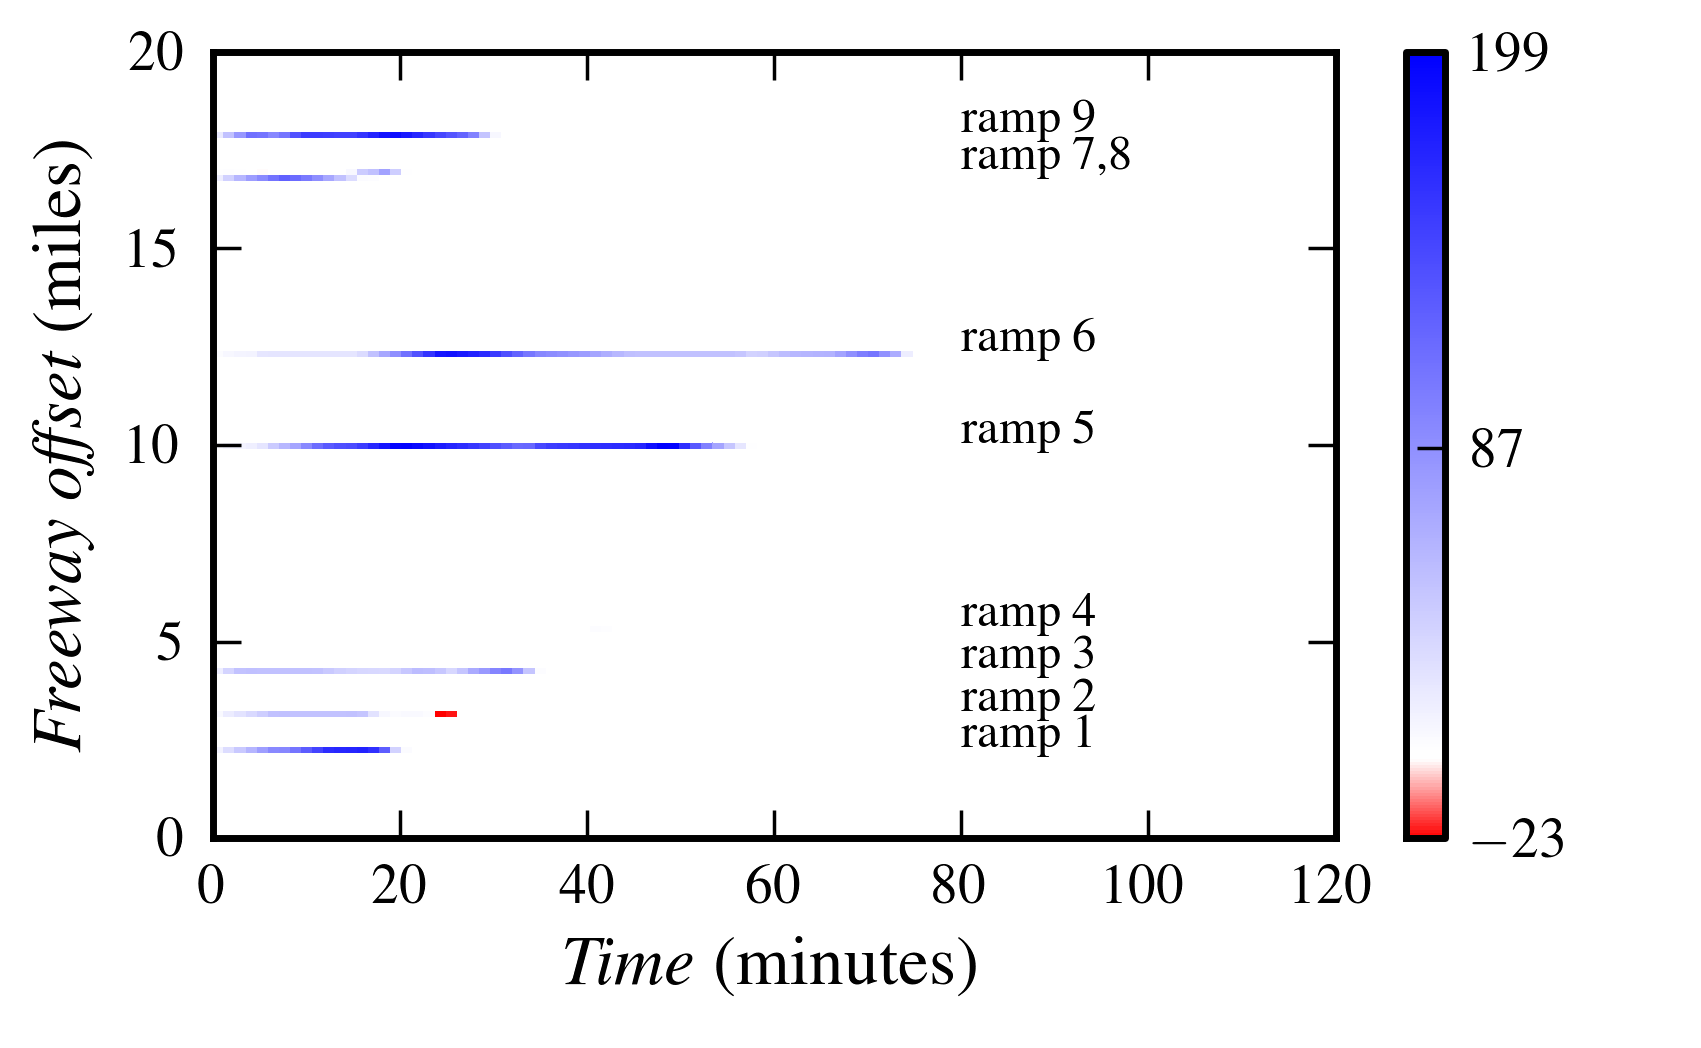
\includegraphics[width=0.45\columnwidth]{images/queuediff}

}

\caption{Profile differences for mainline densities and onramp queues. Evidenced
by the mainly negative differences in the mainline densities and the
mainly positive differences in the onramp queue lengths, the adjoint
ramp metering algorithm effectively limits onramp flows in order to
reduce mainly congestion.\label{fig:long-sim}}
\end{figure}


Figure~\ref{fig:long-sim} shows a difference profile between the
no control simulation and the simulation applying the ramp metering
policy generated from the adjoint method. Negative differences in
Figures~\ref{fig:long-sim-density} and~\ref{fig:long-sim-queue}
indicate where the adjoint method resulted in fewer vehicles for the
specific link and time-step. The adjoint method was successful in
intelligently deciding which ramps should be metered in order to improve
throughput for the mainline.
\begin{figure}
\begin{centering}
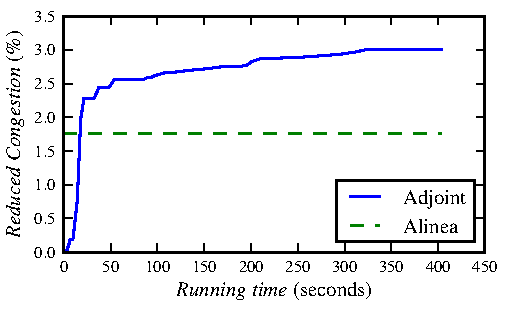
\includegraphics[width=0.65\columnwidth]{images/longsim}
\par\end{centering}

\caption{Performance versus simulation time for freeway network. The results
indicate that the algorithm can run with performance better than Alinea
if given an update time around 15 minutes.}
\end{figure}


Running time analysis shows that the adjoint method can produce beneficial
results running in real time. After just a few gradient steps, the
adjoint method outperforms the Alinea method. Given that the time
horizon of two hours is longer than the period of time one can expect
reasonable estimates of boundary conditions, more practical simulations
with shorter time horizons should permit more gradient steps in a
real-time setting.

While the queue length contains a considerable number of cars in some
onramps for the adjoint method, this problem can be accounted for
by introducing barrier terms into the cost function that limit the
maximum queue length. The Alinea method tested for the I15 network
had no prescribed maximum queue lengths as well, but was not able
to produce significant improvements, while the adjoint method was
more successful in optimizing the road network under the set of constraints.


\subsection{Model predictive control\label{sub:Model-predictive-control}}

To study the performance of the algorithm under noisy input data,
we embed both our adjoint ramp metering algorithm and the Alinea algorithm
inside of a \emph{Model predictive control }(MPC) loop.


\paragraph{Experimental setup}

The MPC loop begins at a time $t$ by estimating the initial conditions
of the traffic on the freeway network and the predicted boundary fluxes
over a certain time horizon $T_{h}$. These values are noisy, as exact
estimation of these parameters is not possible on real freeway networks.
The estimated conditions are then passed to the ramp metering algorithm
to compute an optimal control policy over the $T_{h}$ time period.
The system is then forward simulated over an update period of $T_{u}\le T_{h}$,
using the exact initial conditions and boundary conditions, as opposed
to the noisy data used to compute control parameters. The state of
the system and boundary conditions at $t+T_{u}$ are then estimated
(with noise) and the process is repeated.

A non-negative\emph{ noise factor} is used to study how the adjoint
method and Alinea perform as the quality of estimated data decreases.
The noise factor can be summarized as follows:

\[
\bar{\discrete{}{}}=\discrete{}{}*(1+noise\_factor*R)
\]


where $R$ is a uniformly distributed random variable with mean $0$
and domain $\left[-0.5,0.5\right]$. The noise factor was applied
to both initial and boundary conditions.

Two different experiments were conducted:
\begin{enumerate}
\item \textbf{Real-time I15 South}: MPC is run for the I15 South network
with $T_{h}=27$ minutes and $T_{u}=14$ minutes. A noise factor of
2\% was chosen for the initial and boundary conditions. The number
of iterations was chosen in order to ensure that each MPC iteration
finished in the pre-determined update time $T_{u}$.
\item \textbf{Noise Robustness}: MPC is for over a synthetic network with
length 5 miles and boundary conditions over 50 minutes. The experiments
are run over a profile of noise factors between 1\% and 200\%.
\end{enumerate}

\paragraph{Results}


\subparagraph{Real-time I15 South}

The results are summarized in Figure~\ref{fig:MPC-performance-on}.
The adjoint method applied once to the entire horizon with perfect
boundary and initial condition information serves as a baseline performance
for the other simulations, which had noisy input data and limited
knowledge of predicted boundary conditions. The adjoint method still
performs well under the more realistic conditions of the MPC loop
with noise, resulting in 75\% delay as compared to the no control
scenario as compared to the 71\% delay achieved by the perfect-knowledge
adjoint control. Alinea performed worse than adjoint method, only
achieving a 95\% delay as compared to no control. The results indicate
that under a realistic assumption of a 2\% noise factor in the sensor
information, the ability to consider boundary conditions in producing
ramp metering policies as an improvement upon strictly reactive policies,
such as Alinea.

\begin{figure}
\subfloat[MPC performance on I15 South network.\label{fig:MPC-performance-on}]{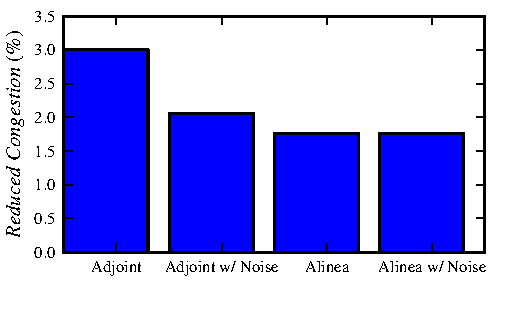
\includegraphics[width=0.45\columnwidth]{images/longmpc}

}\hfill{}\subfloat[MPC performance with increasing sensor noise.\label{fig:Ramp-metering-performance-1}]{\includegraphics[width=0.45\columnwidth]{images/noiseplot}

}
\end{figure}



\subparagraph{Noise Robustness}

Simulation results on the synthetic network with varying levels of
noise are shown in Figure~\ref{fig:Ramp-metering-performance-1}.
The adjoint method is able to outperform the Alinea method when the
noise level is less than 80\%, a reasonable assumption for data provided
by well-maintained loop detectors. As the initial and boundary condition
data deteriorates, the adjoint method becomes useless. Since Alinea
does not rely on boundary data, it is able to produce improvements,
even with severely noisy data. The results indicate that the adjoint
method will outperform Alinea under reasonable noise levels in the
sensor data.

%!TEX root =restart.tex
\section{Conclusions\label{sec:Conclusions}}

This article has detailed a simple framework for finite-horizon optimal control 
methods on a network of scalar conservation laws derived from first 
discretizing the network via the Godunov method, then applying the discrete 
adjoint to this system. To tailor the framework to a specific application, one 
need only provide the partial derivatives of the Riemann solver at a network 
junction as well as the partial derivates of the objective. Furthermore, we 
show that for this class of problems, the sparsity pattern allows the problem 
to be implemented with only linear memory and linear computational complexity 
with respect to the number of state and control parameters. We demonstrate the 
scalability of the approach by implementing a coordinated ramp metering 
algorithm using the adjoint method and applying the algorithm to the I-15 South freeway in California. The algorithm runs in a fraction of real-time 
and produces significant improvements over existing algorithms. The ramp metering algorithm has been fully implemented within Connected Corridors~\cite{CC} system, a project by UC Berkeley and PATH for integrated corridor management, as a component of the traffic simulator module. Future work 
includes investigating decentralized, coordinated control schemes over physical 
networks via the adjoint method to allow traffic control strategies to scale to 
regional-scale networks.

\section{Acknowledgments}\label{sec:ack}

The authors have been supported by the ERC Starting Grant 2010 under the project `TRAffic
Management by Macroscopic Models", the INRIA associated team `Optimal REroute Strategies
for Traffic managEment" and the France-Berkeley Fund under the project `Optimal Traffic Flow
Management with GPS Enabled Smartphones"
\printbibliography

\section*{Nomenclature}

\begin{longtable}{|c|c|c|}
\hline 
Variable  & Space  & Meaning\tabularnewline
\hline 
\hline 
$t$  & $\mathbb{R}_{+}$  & time\tabularnewline
\hline 
$x$  & $\mathbb{R}$  & space\tabularnewline
\hline 
$\nlinks$  & $\mathbb{N}$  & Number of links\tabularnewline
\hline 
$\jns$  &  & Set of junctions\tabularnewline
\hline 
$\links=\left[1,\nlinks\right]$  & $\mathbb{N}^{N}$  & Set of links\tabularnewline
\hline 
$L_{\link}$  & $\mathbb{R}_{+}$  & Length of link $\link\in\links$\tabularnewline
\hline 
$\cvar_{i}\left(t,x\right)$  & $\mathbb{R}_{+}\times\left]0,L_{i}\right[\rightarrow\mathbb{R}$  & conserved quantity for link $\link\in\links$ as function of $x$\tabularnewline
\hline 
$\initstate$  & $BV\cap L_{\text{loc}}^{1}$  & continuous intialial condition\tabularnewline
\hline 
$\dvar_{\link}^{\tind}$  & $\mathbb{R}$  & discrete conserved quantity for link $i$ at time-step $k$\tabularnewline
\hline 
$f(\cvar)$  & $f:\mathbb{R}\rightarrow\mathbb{R}$  & flux function\tabularnewline
\hline 
$\initstate$  & $\mathbb{R}$  & Riemann data\tabularnewline
\hline 
$\cvar^{-}$  & $\mathbb{R}$  & Left state of the Riemann data\tabularnewline
\hline 
$\cvar^{+}$  & $\mathbb{R}$  & Right state of the Riemann data\tabularnewline
\hline 
$\bar{x}$  & $\mathbb{R}$  & Point of discontinuity in Riemann problem\tabularnewline
\hline 
$\ssvar$  & $\mathbb{R}$  & Self-similar solution of the Riemann problem\tabularnewline
\hline 
$n_{J}$  & $\mathbb{N}$  & Number of incoming links at a junction J\tabularnewline
\hline 
$m_{J}$  & $\mathbb{N}$  & Number of outgoing links at a junction J\tabularnewline
\hline 
$\Inc\left(\jn\right)=\tuple{\jlink{\jn}1}{\jlink{\jn}{\ninc_{\jn}}}\subset\links$  &  & Set of incoming links at a junction J\tabularnewline
\hline 
$\Out\left(\jn\right)=\tuple{\jlink{\jn}{\ninc_{\jn}+1}}{\jlink{\jn}{\ninc_{\jn}+\nout_{\jn}}}\subset\links$  &  & Set of outgoing links at a junction J\tabularnewline
\hline 
$\jup{\link}\in\jns$  &  & Upstream junction for the link $\link\in\links$\tabularnewline
\hline 
$\jdown{\link}\in\jns$  &  & Downstream junction for the link $\link\in\links$\tabularnewline
\hline 
$\RS$  & $\mathbb{R}^{m+n}\rightarrow\mathbb{R}^{m+n}$  & Riemann Solver\tabularnewline
\hline 
$\trace{\cvar}_{\link}$  & $\mathbb{R}^{m+n}$  & Trace for a link $i$ at the junction\tabularnewline
\hline 
$\Delta t$  & $\mathbb{R}$  & Time grid size\tabularnewline
\hline 
$\Delta x$  & $\mathbb{R}$  & Space grid size\tabularnewline
\hline 
$t^{\tind}=k\Delta t$  & $k\in\mathbb{N}$  & Time grid points\tabularnewline
\hline 
$t^{\xind}=l\Delta x$  & $l\in\mathbb{Z}$  & Space grid points\tabularnewline
\hline 
$\lambda^{\max}$  & $\mathbb{R}$  & Wave speed\tabularnewline
\hline 
$\juncstate{\jn}{\tind}$  & $\mathbb{R}^{m_{\jn}+n_{\jn}}$  & state variables at a junction $\jn\in\jns$ at a time-step $\tind$\tabularnewline
\hline 
$T$  & $\mathbb{N}$  & Number of time steps\tabularnewline
\hline 
$\junctrace{\jn}{}$  & $\mathbb{R}^{m_{\jn}+n_{\jn}}$  & solution of $\RS$ at a junction $\jn\in\jns$ at a time-step $\tind$\tabularnewline
\hline 
$\junccon{\jn}{\tind}$  & $\mathbb{R}^{\ncontrols_{\jn}}$  & control variables at a junction $\jn\in\jns$ at a time-step $\tind$\tabularnewline
\hline 
$\syseq_{\link}^{\tind}$  & $\mathbb{R}^{\nlinks\ntime}\times\mathbb{R}^{\ncontrols\ntime}$  & update equation\tabularnewline
\hline 
$\cost$  & $\mathbb{R}^{\nlinks T}\times\mathbb{R}^{N_{\control}T}$  & cost function\tabularnewline
\hline 
$\lambda$  & $\mathbb{R}^{\nlinks\ntime}$  & adjoint variable\tabularnewline
\hline 
$D_{\state}$  & $\mathbb{N}$  & maximum junction degree on the network \tabularnewline
\hline 
$D_{\control}$  & $\mathbb{N}$  & maximum number of constraints \tabularnewline
\hline 
$\splitratio_{2\link}^{\tind}$  & $[0,1]$  & offramp split ratio \tabularnewline
\hline 
$\boundaryDemand{2\link-1}{\tind}$  &  & flux demand at the boundary of onramp $2\link-1$\tabularnewline
\hline 
$\barrierTerm$  &  & barrier penalty coefficient \tabularnewline
\hline 
$\demand_{2\left(\link-1\right)}$  &  & demand on the link $2(i-1)$ \tabularnewline
\hline 
$\rampDemand_{2\link-1}^{\tind}$  &  & demand from onramp $2\link-1$\tabularnewline
\hline 
$\supply_{2\link}^{\tind}$  &  & supply on the link $2i$ \tabularnewline
\hline 
$\ffspeed_{\link}$  & $\mathbb{R}_{+}$ & free flow speed for link $\link$\tabularnewline
\hline 
$\congspeed_{\link}$  & {[}0,1{]}  & congestion speed $\link$\tabularnewline
\hline 
$p_{2\left(\link-1\right)}$  & {[}0,1{]}  & merging parameter \tabularnewline
\hline 
\end{longtable}


\end{document}
